\documentclass[
	12pt,
    a4paper,
    egregdoesnotlikesansseriftitles, % Überschriften haben gleichen Font wie restlicher Text
    toc=chapterentrywithdots,
    oneside, openany,
    % twoside,openright,
    titlepage,
    parskip=half,
    headings=normal,  % reduces heading size
    listof=totoc,
    bibliography=totocnumbered,
    index=totoc,
    captions=tableheading,  % caption below table
    % chapterprefix,
    listof=flat,
    numbers=noenddot, % kein Punkt nach Nummerierung im Inhaltsverzeichnis
    final]
    {scrbook}
    
% details about your thesis
\newcommand{\titel}{UML Class Diagrams: A Comprehensive Study of Aggregation, Composition, Dependencies, Interfaces, and Inheritance}
\newcommand{\artderarbeit}{Studienarbeit}  % {Bachelorarbeit,Masterarbeit}
\newcommand{\autor}{Ronny Pollak}
\newcommand{\modul}{Systementwurf und Systemdokumentation mit UML und SysML} 
%\newcommand{\modulzusatz}{Strategien,\,Architekturen\,und\,Algorithmen}
\newcommand{\matrikelnr}{123\,4567}
\newcommand{\dozent}{Prof.\,Dr.-Ing.\,Dipl.-Inf. Axel Hein}
\newcommand{\abgabedatum}{13.01.2023}
\newcommand{\keywords}{key, words}
%\newcommand{\studentname}{key, words}
%\newcommand{\studentMatnr}{key, words}
\newcommand{\studentStudiengang}{Master Informatik}


% custom head and foot
\usepackage[automark]{scrlayer-scrpage}
\pagestyle{scrheadings}
\ihead{\headmark}
\chead{}
\ohead{\pagemark}
\renewcommand*\chaptermarkformat{\chapappifchapterprefix{\ }% 
  \thechapter.\enskip}
% anderenfalls zu viel Abstand von Titeln zu oberem Seitenrand
\RedeclareSectionCommand[afterindent=false,beforeskip=0pt]{chapter}

\RedeclareSectionCommand[tocindent=0pt]{section}
\RedeclareSectionCommand[tocindent=0pt]{subsection}
%\RedeclareSectionCommand[tocnumwidth=70pt]{chapter}

\usepackage{scrhack}

% other packages
\usepackage[utf8]{inputenc}
\usepackage[T1]{fontenc}
\usepackage{lmodern,relsize,textcomp,csquotes}
\usepackage{amsmath,amsfonts}
\usepackage[ngerman,english]{babel}  % flip for German thesis
\usepackage[final]{graphicx}
\usepackage{setspace,geometry,xcolor}
\usepackage{makeidx}
\usepackage{paralist,ifthen,todonotes}
\usepackage{url}
\usepackage[toc]{glossaries}
\usepackage{pdfpages}

% table setup
\usepackage{longtable}
\usepackage{array}
\usepackage{ragged2e}
\usepackage{lscape}


\usepackage{hyperref}


% configure your listings style
\usepackage{listings}
\lstset{
	tabsize=3,
	extendedchars=true,
	frame=single,
	showstringspaces=true,
	numbers=left,
	numberstyle=\small,
	breakautoindent=true
}

% page setup
% \setlength{\topskip}{\ht\strutbox}
\geometry{paper=a4paper,left=2.5cm,top=3.0cm,bindingoffset=.8cm}
\onehalfspacing
%\frenchspacing
%\linespread{1.25} % NEU
\clubpenalty = 10000
\widowpenalty = 10000 
\displaywidowpenalty = 10000

% some commands
\newcommand{\ua}{\mbox{u.\,a.\ }}
\newcommand{\zB}{\mbox{z.\,B.\ }}
\newcommand{\dahe}{\mbox{d.\,h.,\ }}
\newcommand{\bzw}{\mbox{bzw.\ }}
\newcommand{\bzgl}{\mbox{bzgl.\ }}
\newcommand{\eg}{\mbox{e.\,g.\ }}
\newcommand{\ie}{\mbox{i.\,e.\ }}
\newcommand{\wrt}{\mbox{w.\,r.\,t.\ }}
\newcommand{\etal}{\mbox{\emph{et.\,al.\ }}}


% TODO remove if not needed...
\usepackage{blindtext}
\usepackage{todonotes}

% NEU musste für Bilder eingefügt werden
\usepackage{graphicx}
% NEU:damit Bilder nicht rumfloaten und an einer BESTIMMTEN Stelle sind -> [H]
\usepackage{float}

% Biblatex
\usepackage[backend=bibtex,style=alphabetic]{biblatex}
\addbibresource{refs.bib}

% load glossary entries
\makenoidxglossaries
\loadglsentries{glossary}

%\counterwithout{figure}{chapter}
% um nicht die Nummer des Kapitels bei der Figure Nummerierung zu stehen haben

\sloppy
%damit \textt nicht über die zeile hinaus geht

\begin{document}
\setcounter{secnumdepth}{3}  % numerate subsections
\setcounter{tocdepth}{2}  % ...but don't include them in toc


\frontmatter
\thispagestyle{empty}
\pdfbookmark[1]{Cover}{cov}
\begin{titlepage}

\begin{center}


\includegraphics[width=\linewidth]{figures/TH-Nuernberg-RGB.png}\\[1cm]
\LARGE{Fakultät Informatik}\\[2cm]

\huge
\textbf{\titel}\\[1cm]
%
\Large
\modul\\%[1cm]
\small


\vfill
\normalsize
%\newcolumntype{x}[1]{>{\raggedleft\arraybackslash\hspace{0pt}}p{#1}}
\begin{tabular}{rl}%{6cm}p{7.5cm}}
    \rule{0mm}{1ex}\textbf{Vorgelegt von:} & \autor \\
	\rule{0mm}{1ex}\textbf{Matrikelnummer:} & \hspace*{-0.5em}\begin{tabular}[t]{r}\matrikelnr\end{tabular} \\ 
	\rule{0mm}{1ex}\textbf{Studiengang:} & \studentStudiengang \\
	\rule{0mm}{1ex}\textbf{Dozent:} & \dozent \\ 
	\rule{0mm}{1ex}\textbf{Abgabedatum:} & \abgabedatum \\ 
\end{tabular} 		


\end{center}


%\vspace{-0.5cm}
%\singlespacing
%\small
%\noindent Dieses Werk einschließlich seiner Teile ist \textbf{urheberrechtlich geschützt}.
%Jede Verwertung außerhalb der engen Grenzen des Urheberrechtgesetzes ist ohne Zustimmung des Autors unzulässig und strafbar.
%Das gilt insbesondere für Vervielfältigungen, Übersetzungen, Mikroverfilmungen sowie die Einspeicherung und Verarbeitung in elektronischen Systemen.

\end{titlepage}

\tableofcontents

\listoffigures
\clearpage %\cleardoublepage % https://golatex.de/wiki/%5Ccleardoublepage

\listoftables
\clearpage %\cleardoublepage

\renewcommand{\lstlistlistingname}{List of Listings}  % change for German thesis
%\lstlistoflistings
\clearpage %\cleardoublepage

\mainmatter

\chapter{Introduction}

%TODO Add citation of levin

\section{Motivation}
This comprehensive study focuses on the various types of more complex relationships that can be represented in UML class diagrams. 
These relationships include \emph{aggregation}, \emph{composition}, \emph{dependencies}, \emph{interfaces}, \emph{abstract} classes and \emph{inheritance}. 
Each of these relationships reflects a specific type of connection between classes and serves a unique purpose in the design and implementation of object-oriented systems. 
The following sections define and provide examples of each of these relationships.
This paper extends the work of Levin [insert paper citation] and does not delve into the basic concepts, that will be mentioned in the next section, in great detail. 
The focus is on furthering the research and providing examples to support the points made.
The examples will build on a hypothetical delivery drone which is introduced in Levin's [citation] paper.
By the end of this paper, readers should have a thorough understanding of the role of complex relationships in UML class diagrams and how to effectively use them to model object-oriented systems.

%TODO Levin zitieren

\section{Introduction to UML class diagram}
UML (Unified Modeling Language) class diagrams are a visual representation of the static structure of an object-oriented system. 
They are commonly used in software engineering to model the classes, attributes, operations, and relationships within a system, as well as the interactions between these components. 
A class in UML is a blueprint for an object, which is a runtime instance of that class. 
Classes are represented by rectangles in UML class diagrams, and typically contain three compartments: 
\begin{itemize}
	\item Class name
	\item \emph{Attributes}
	\item \emph{Operations}
\end{itemize}
Attributes are properties or characteristics of the class and are typically displayed in the middle compartment of the rectangle.
Operations are the behaviors or actions that the class can perform and are displayed in the bottom compartment of the rectangle.
In programming terms, these would be the variables and the methods or functions.
Basic relationships are called \emph{associations}. 
An Association indicates that one class has a reference to another class. \cite[p. 108-111]{uml}
The association is shown using a solid line with an open arrow at one end, indicating the direction of the relationship. \cite[p. 142-143]{uml}

\chapter{Aggregation and Composition}
Aggregation and composition are two types of relationships that can be represented in a UML class diagram. 
They both are subtypes of associations and represent a relationship between two classes in which one class has a reference to another class, but they differ in the degree to which the lifetime of the referenced class is tied to the referencing class.
%angeblich Plagiat

\section{Aggregation}
Aggregation is a weaker form of relationship than composition and is indicated in a UML class diagram by a solid line with a hollow diamond at one end. 
It represents a "part-of" relationship between two classes, in which the referencing class (the class with the diamond) is composed of one or more instances of the referenced class (the class on the other end of the line).
The referencing class consists of the referenced class.
However, the lifetime of the referenced class is independent of the referencing class.
If the referencing class is destroyed, the referenced class may continue to exist.
This means that the part of a whole can exist without the whole.
In aggregation, as in associations, every combination of multiplicities is possible. \cite[p. 153]{uml}


\begin{figure}[h]
	\centering
	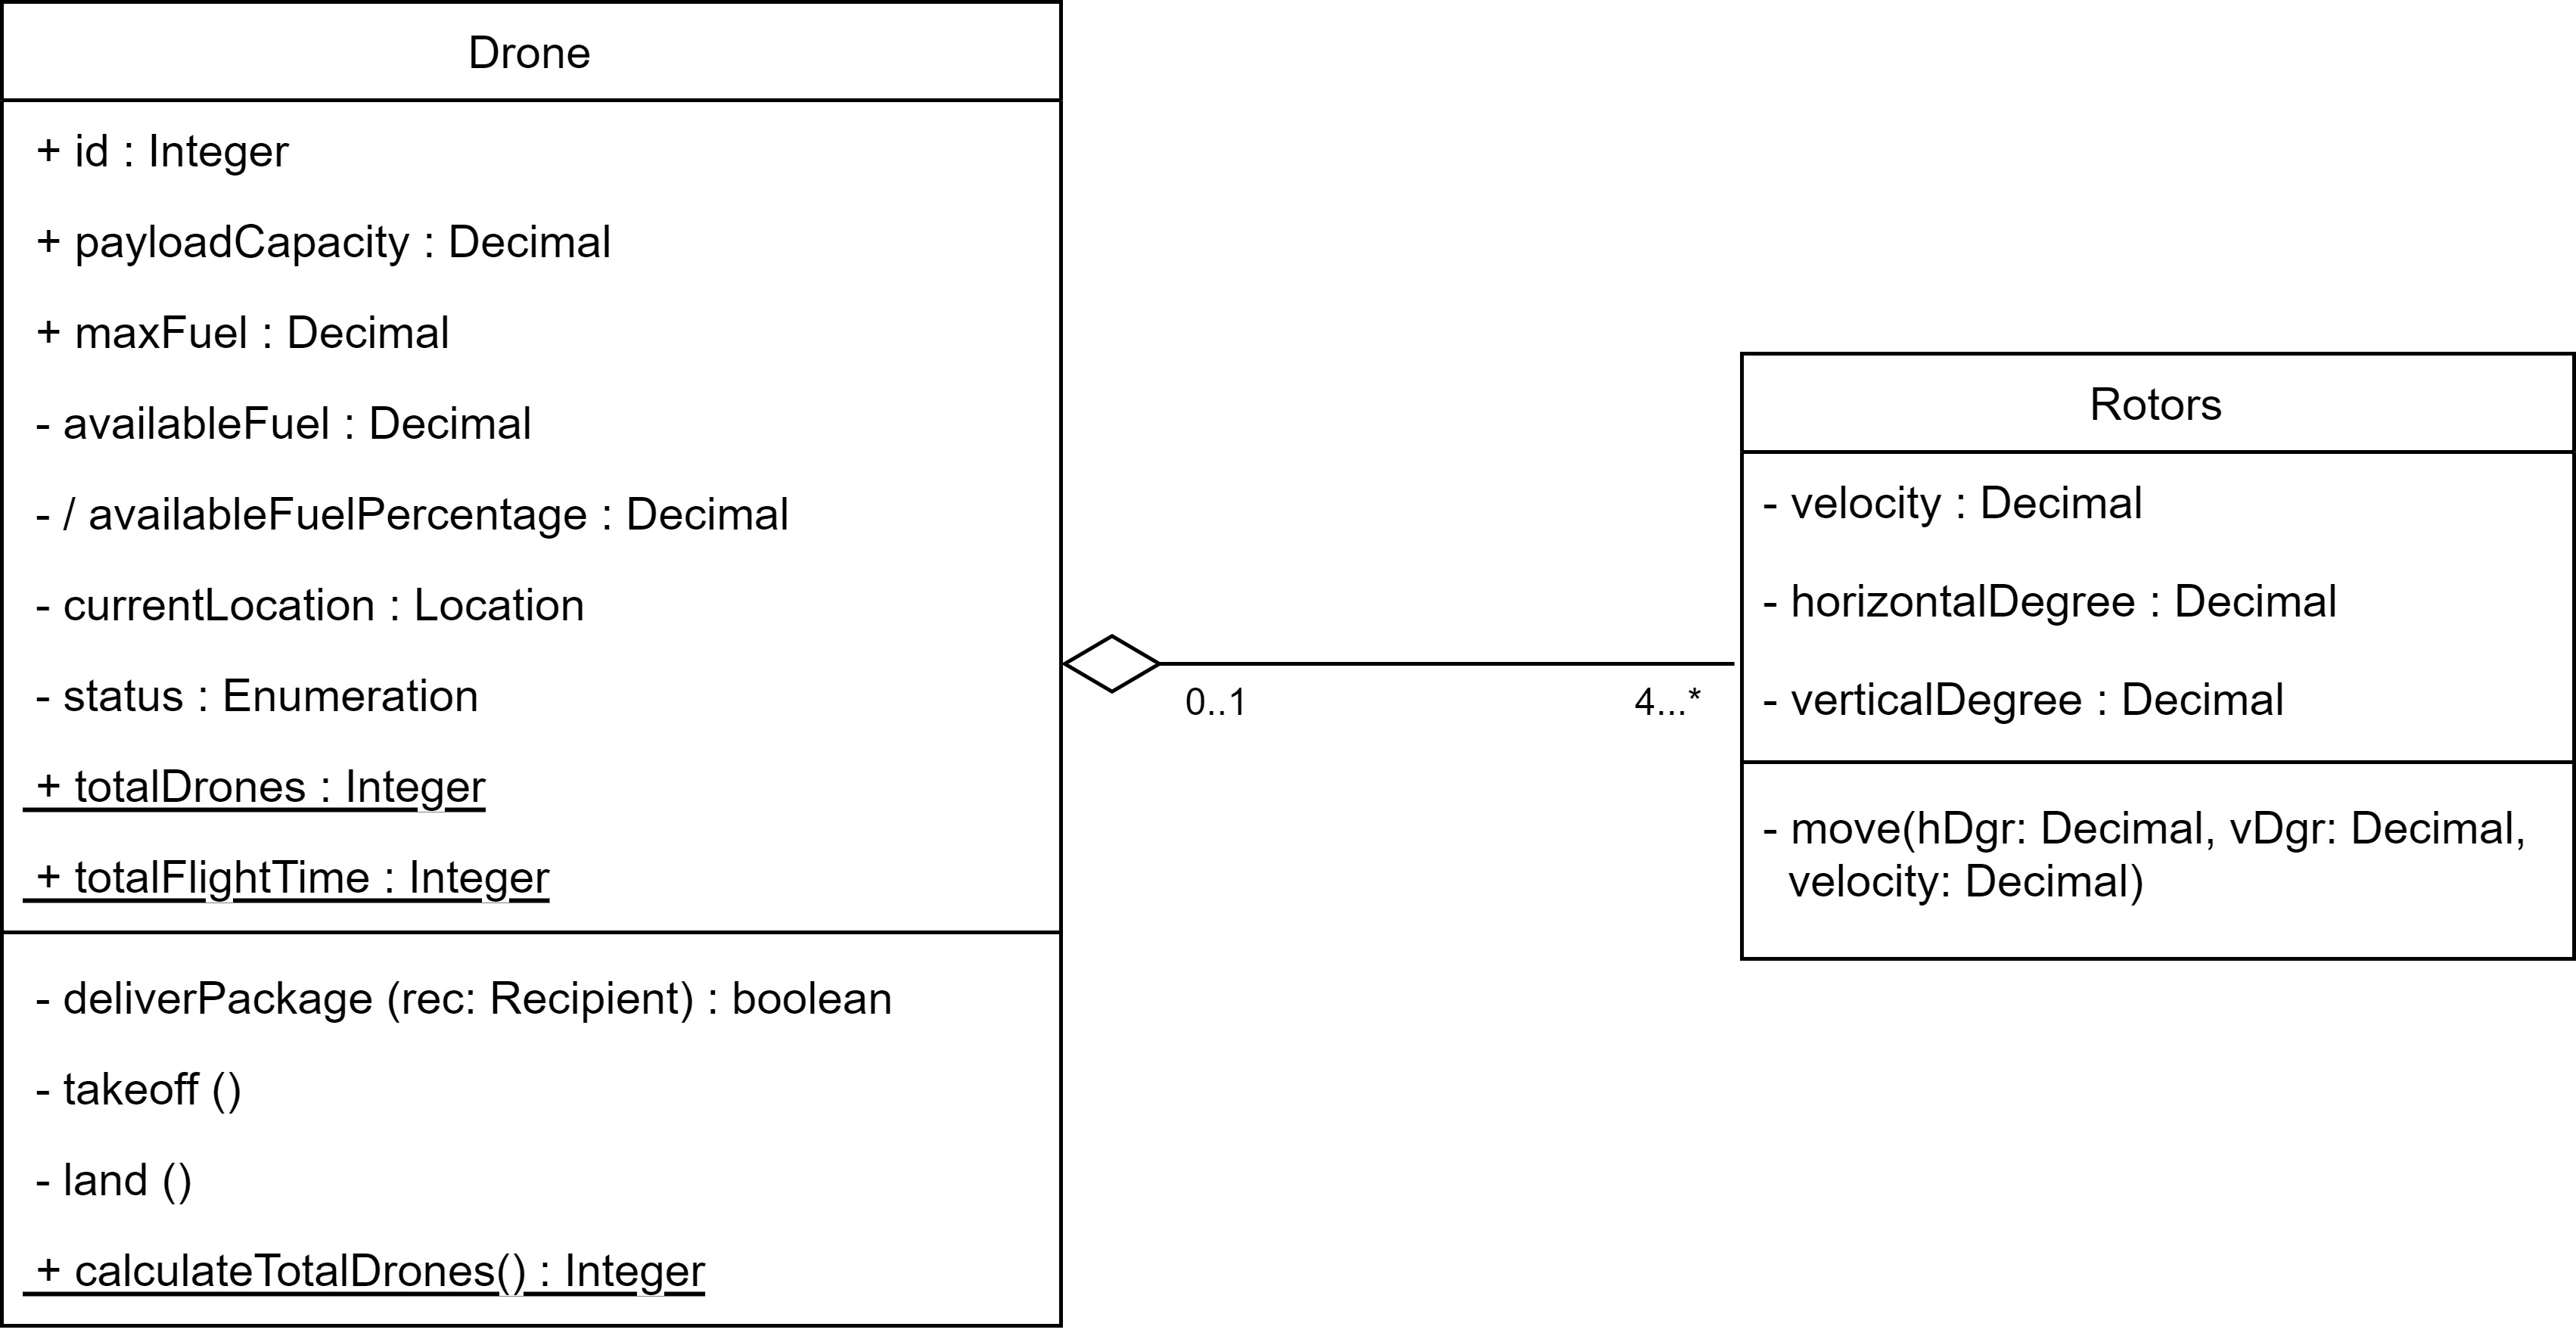
\includegraphics[width=0.8\textwidth]{figures/aggr_comp/aggr.jpg}
	\caption[Example aggregation]{Example of an aggregation}
	\label{fig:aggregation_example} 
\end{figure}


An example of an aggregation relationship involving a \texttt{Drone} class and a \texttt{Rotor} class is demonstrated in Figure \ref{fig:aggregation_example}. 

%TODO Text an neue operationen anpassen und send drontoRecipient rausnehmen
The \texttt{Drone} class includes a private operation, \texttt{sendDroneToRecipient()}, which involves tasks such as navigating to the recipient's location, verifying the delivery details, and safely delivering the package.
The \texttt{Rotor} class, on the other hand, contains a private operation, \texttt{move()}, which is called by the \texttt{Drone} class's \texttt{sendDroneToRecipient()} operation and three private attributes, \texttt{velocity}, \texttt{horizontalDegree}, and \texttt{verticalDegree}, which control the movement of the drone in the air. 

The \texttt{Drone} class serves as the referencing class in this aggregation relationship and requires at least four \texttt{Rotor} instances to function properly. 
However, the drone has the capacity to utilize up to eight rotors at a time, as there are eight available slots for rotors on the drone. 
Each \texttt{Rotor} instance can be part of one or no drones at a given time.

If the \texttt{Rotor} instances become worn down or the weather conditions change, they can be replaced with new or specialized rotors. 
The destruction of a \texttt{Rotor} instance does not affect the existence of the \texttt{Drone}, and conversely, the destruction of a \texttt{Drone} instance does not affect the \texttt{Rotor} instances.


\section{Composition}

In a UML class diagram, composition is a stronger form of relationship than aggregation and is represented by a solid line with a solid diamond at one end pointing toward the composite class. It represents a whole-part relationship between two classes, in which the whole class, known as the composite, is composed of one or more instances of the part class, known as the component.

The composite class is responsible for the lifecycle of the component class, meaning that the composite class creates and destroys the component class as needed. The component class cannot exist independently of the composite class and is tightly bound to the composite class. This is in contrast to an aggregation relationship, where the component class can exist independently of the aggregate class.

The multiplicities available for use in a composition relationship are restricted compared to those in an aggregation relationship. While a whole can have any number of parts, a part can only contribute to one whole. The multiplicity indicated by the solid diamond in a composition relationship is fixed at 0, 0..1, or 1. In many cases, the multiplicity is left out, which implies a multiplicity of 1. A multiplicity of 0 does not make sense in a composition relationship, and a multiplicity of 0..1 means that the parts are capable of existing independently for a certain period of time.
 \cite[p. 153-154]{uml}

\begin{figure}[h]
\centering
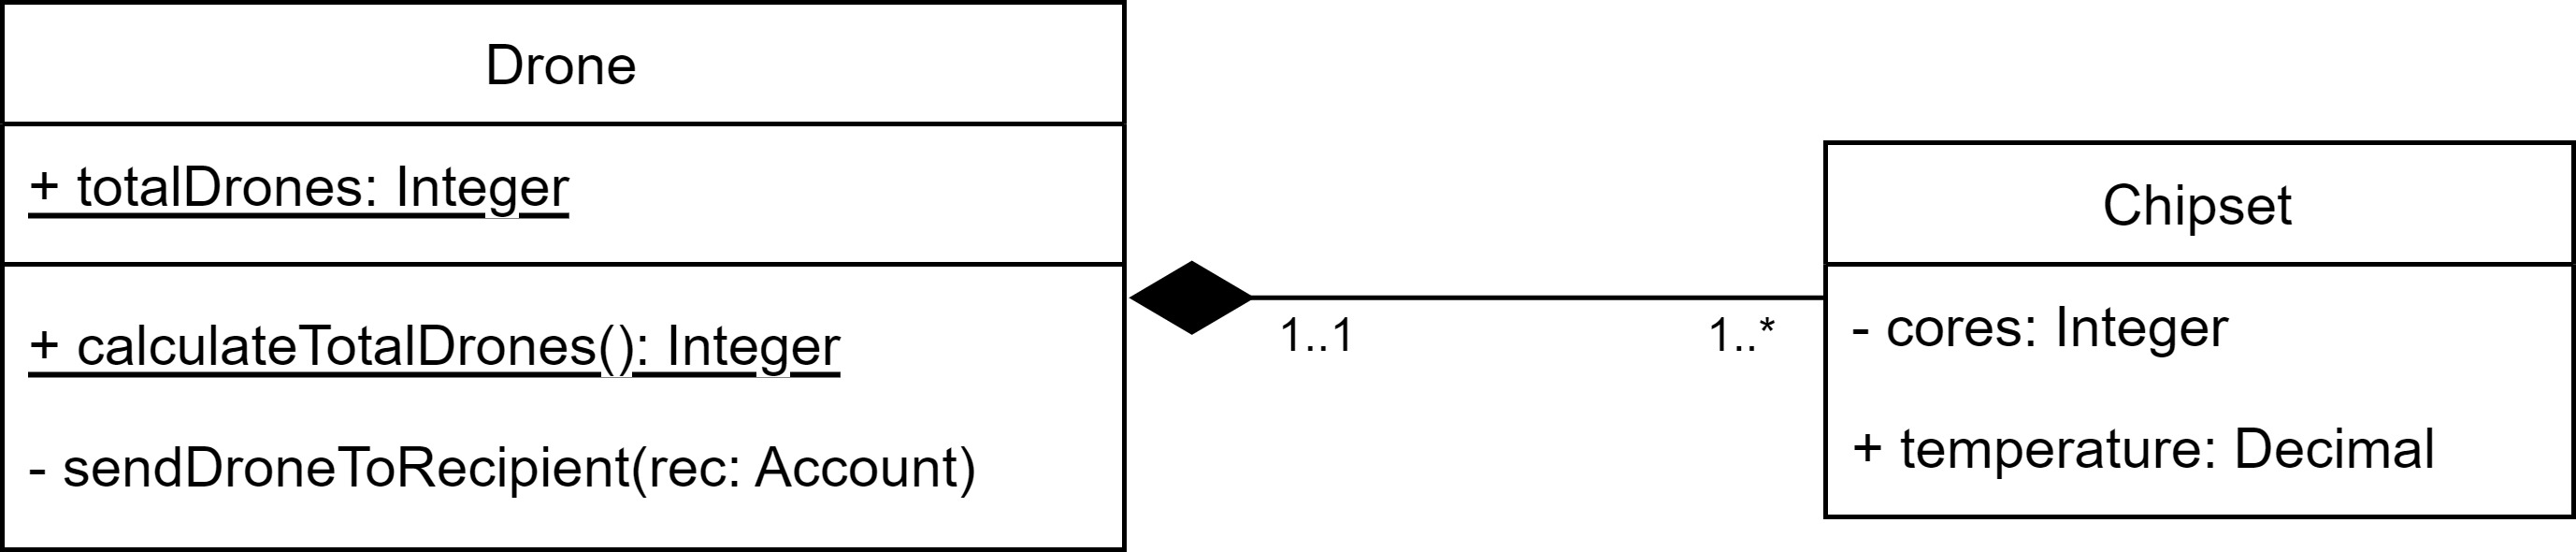
\includegraphics[width=0.8\textwidth]{figures/aggr_comp/comp.jpg}
\caption[Example composition]{Example of a composition}
\label{fig:composition_example}
\end{figure}


In Figure \ref{fig:composition_example}, an example of a composition relationship between the \texttt{Drone} class and the \texttt{Chipset} class is displayed. The \texttt{Chipset} class contains the private attribute \texttt{cores}, which stores information about the number of cores present in the chipset, and the public attribute \texttt{temperature}, which reflects the temperature of the chipset. As a vital component of the drone, the chipset is responsible for processing data and issuing commands to other parts of the drone. Without a functioning chipset, the drone would be unable to operate.

This design also incorporates an anti-theft concept, in which each chipset is uniquely bound to a specific drone. The number of chipsets used by the drone may vary based on their efficiency and the desired level of efficiency for the drone.


\chapter{Dependencies}
%In UML, a dependency is a relationship between two elements in which one element (the client) uses or depends on another element (the supplier) for specification or implementation.
%The dependency represents a semantic or structural relationship between the supplier and the client, indicating that the client is dependent on the supplier in some way.
%A dependency indicates that the connection between the two elements is at a higher level of abstraction than an association relationship.
%Dependencies can be represented in various UML diagrams, including class diagrams, component diagrams, deployment diagrams, and use-case diagrams. 
%To represent a dependency in a UML diagram, a dashed line with an open arrow pointing from the client to the supplier is used. 
%In some cases, stereotypes may be used to show the precise nature of the dependency. \cite[p. 159-160]{uml}
In UML, a dependency relationship is a semantic or structural link between two elements, where one element (the client) uses or depends on the other element (the supplier) for its specification or implementation. 
A dependency indicates that the connection between the two elements is at a higher level of abstraction than an association relationship.
This dependency relationship can be represented in different types of UML diagrams, such as class, component, deployment, or use-case diagrams. 
The notation for a dependency is a dashed line with an open arrow pointing from the client to the supplier.
Stereotypes may also be used to specify the specific type of dependency. \cite[p. 159-160]{uml}

The following Table \ref{tab:dependencies} shows the different types of dependencies, their stereotype, and a description.

%TODO Binding rausnehmen?
\vspace{1em}
{\RaggedRight
\begin{longtable} {|p{3.5cm}|p{3.25cm}|p{6.5cm}|}
		\hline
		\textbf{Type of dependency} & \textbf{Stereotype} & \textbf{Description} \\
		\hline
		Abstraction & «abstraction», «derive», «refine», or «trace» & Relates two model elements, or sets of model elements, that represent the same concept at different levels of abstraction, or from different viewpoints  \\ 
		\hline
		Realization & «realize» & 	Indicates that the client model element is an implementation of the supplier model element, and the supplier model element is the specification \\ 
		\hline
		Substitution & «substitute» & Indicates that the client model element takes the place of the supplier; the client model element must conform to the contract or interface that the supplier model element establishes  \\ 
		\hline
		Usage & «use», «call», «create», «instantiate», or «send» & Indicates that one model element requires another model element for its full implementation or operation  \\ 
		\hline
	\caption[Types of dependencies]{Types of dependency \cite{ibm_dependencies} \cite{uml}}
	\label{tab:dependencies}
\end{longtable}
}

In the following sections, the different types of dependencies will be explained with examples.

\section{Usage}
%In the context of modeling and software development, a usage relationship is a dependency in which one element (client) requires another element (supplier) for its full implementation or operation. 
%The client element is considered incomplete without the supplier element. 
%The usage relationship is represented using the stereotype \texttt{<<use>>} and is depicted using a dashed line with an arrow pointing from the client element to the supplier element. 
%The client and supplier elements can be any named elements in the model. 
%The difference between a usage relationship and a normal dependency relationship is minimal, with the main distinction being that the \texttt{<<use>>} stereotype may be used to specify that the dependency is specifically related to the actual use of the supplier element. \cite[p. 161]{uml}


A usage relationship in UML is a dependency in which one element (the client) requires another element (the supplier) for its proper operation or implementation. 
It's represented a using a dashed line with an arrow pointing from the client to the supplier element, and the stereotype \texttt{<<use>>} may be used to indicate it's specifically related to the actual use of the supplier element. 
The difference between a usage relationship and a normal dependency relationship is minimal, with the main distinction being that the \texttt{<<use>>} stereotype may be used to specify that the dependency is specifically related to the actual use of the supplier element. \cite[p. 161]{uml}

\vspace{1em}
\begin{minipage}{\linewidth}
	\centering
	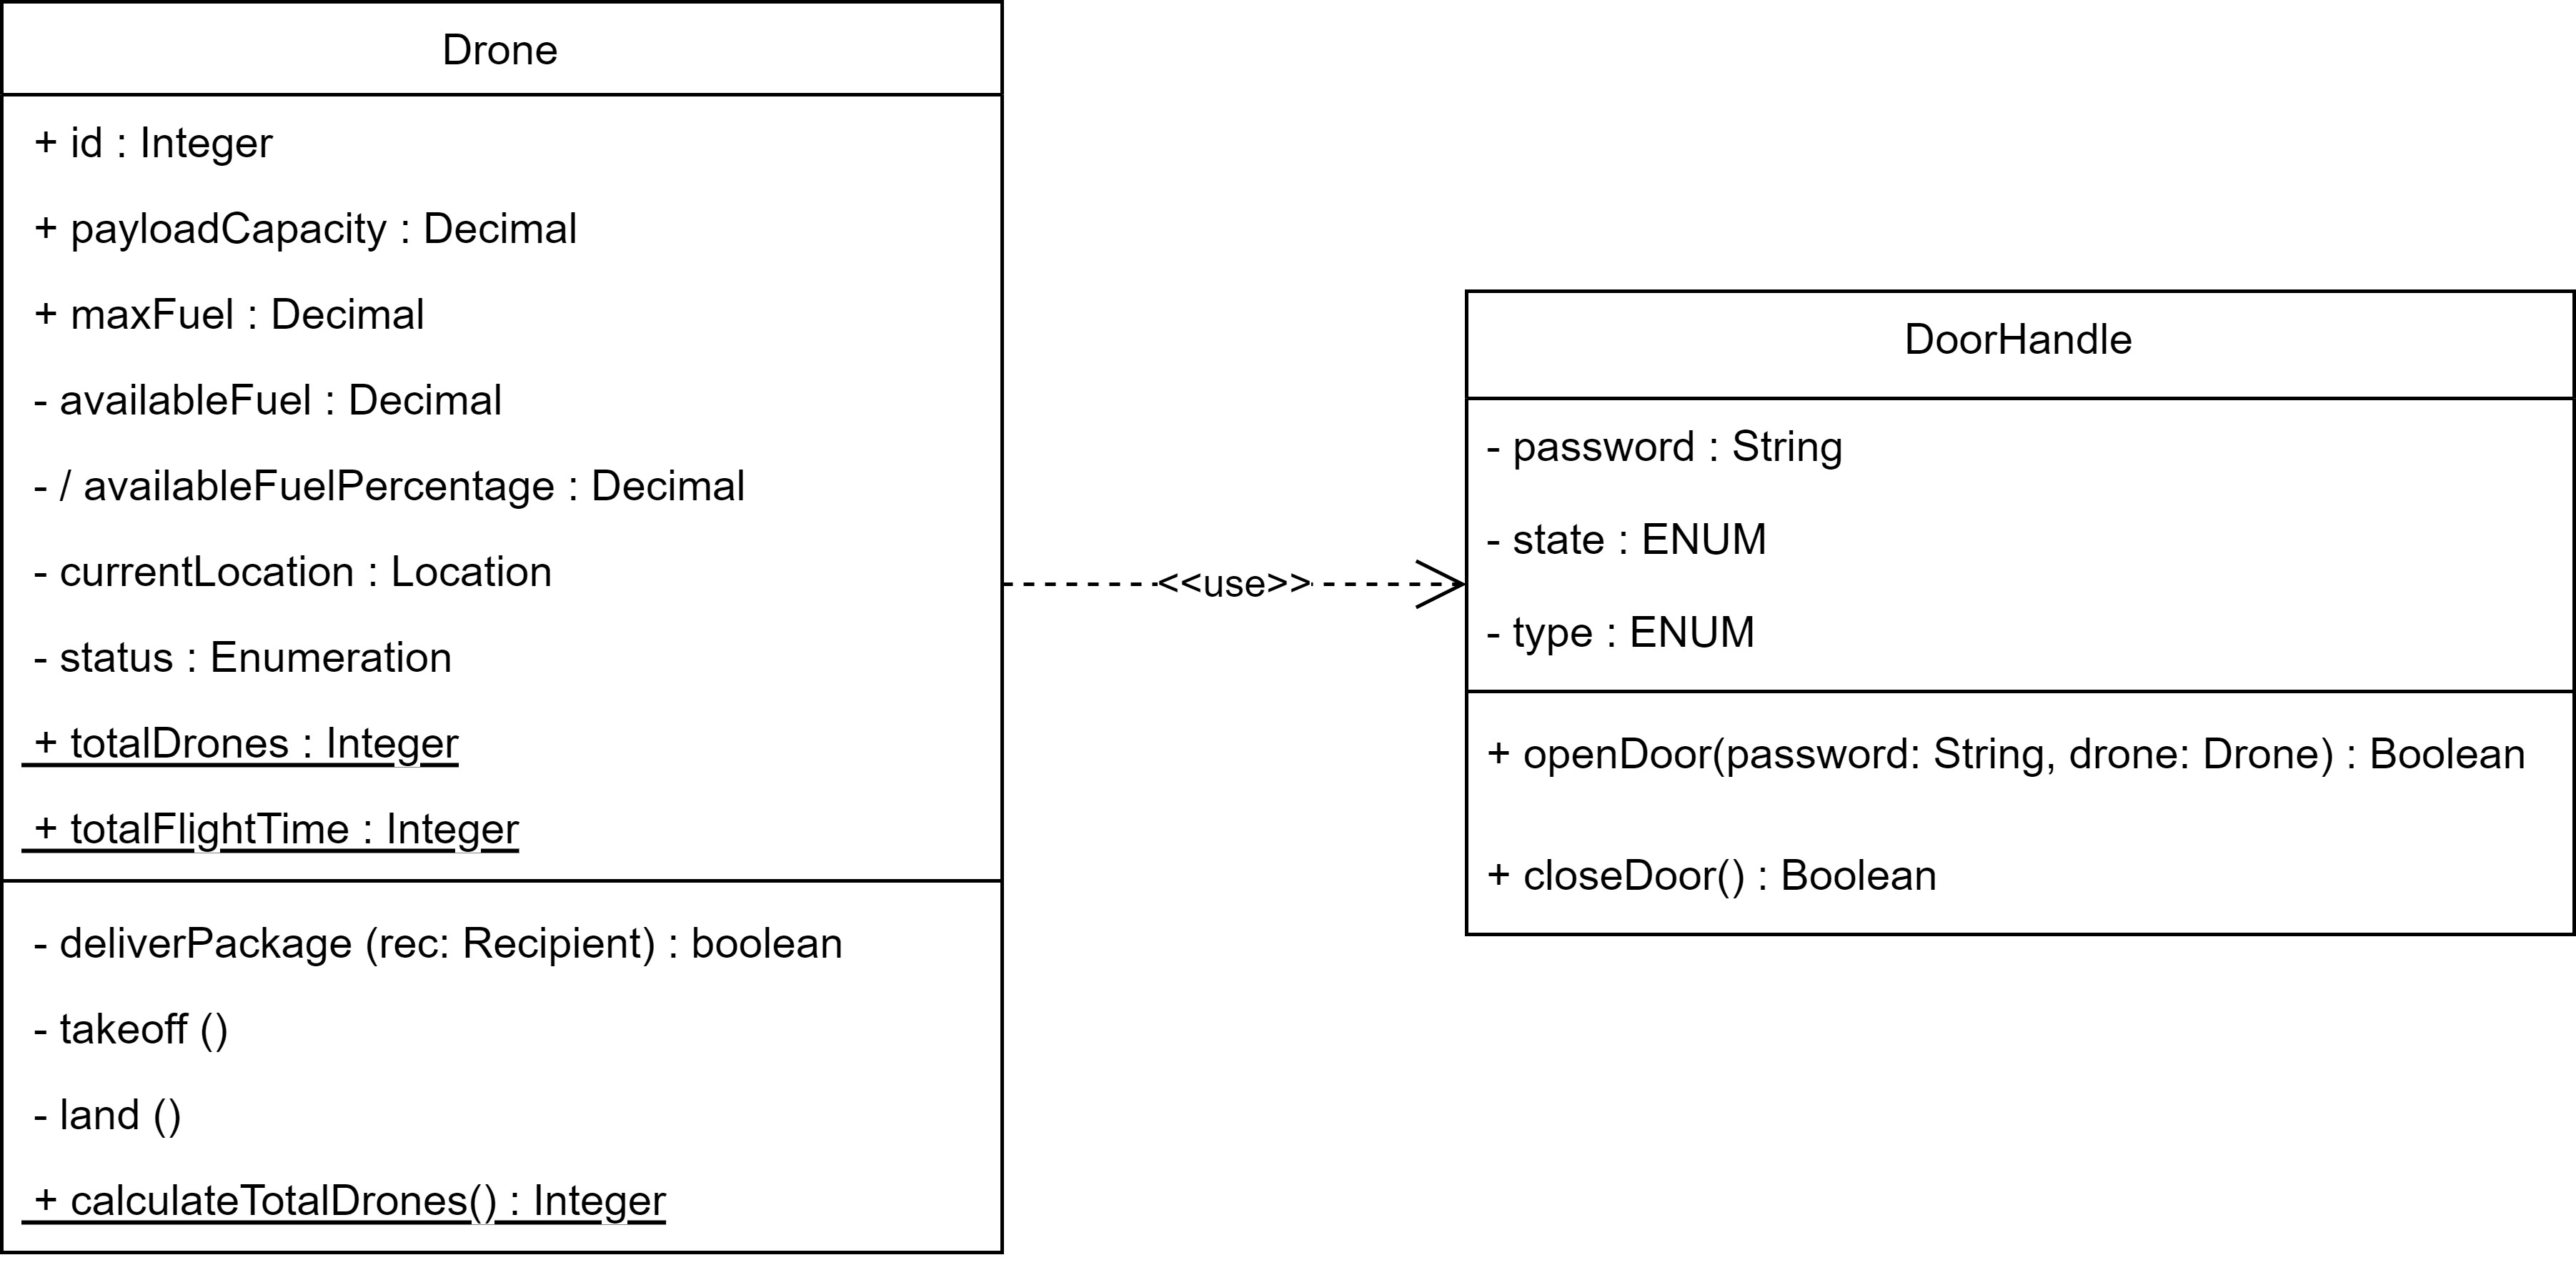
\includegraphics[width=0.8\textwidth]{figures/dependencies/usage.jpg}
	\captionof{figure}[Example usage]{Example of usage}
	\label{fig:usage_example}
\end{minipage}


In Figure \ref{fig:usage_example}, an example of a usage relationship between the \texttt{Drone} class and the \texttt{DoorHandle} class is displayed. The \texttt{DoorHandle} class contains the private attribute \texttt{type}, which stores information about the type of door handle, and the public operation \texttt{open()} which allows the door to be opened with a password.
This operation also utilizes the \texttt{state} enumeration to store the current state of the door handle, including \texttt{open}, \texttt{closed}, and \texttt{invalid} states.
It enters the invalid state if an error occurs while opening or closing the door

The DoorHandle is built into various types of doors and is responsible for providing a mechanism for opening the door. 
The drone uses the DoorHandle to open doors as part of its delivery tasks and drops off the packages in the desired place. 
This can include houses, garages, or shacks. 
To open a door, the drone calls the public \texttt{open()} operation of the DoorHandle class and passes in the password for the door. 
If the password is correct, the door is opened and the Drone class can complete its delivery. 
Afterwards, the door will be closed again with the public operation \texttt{closeDoor()}.
The Drone class is the client that uses the DoorHandle class as the supplier.

%TODO is this useless?
%This usage relationship between the Drone and DoorHandle classes can be represented with a directed line with an arrowhead pointing from the Drone class to the DoorHandle class and the stereotype <<use>>. The Drone class is the client that uses the DoorHandle class, and the DoorHandle class is the supplier that provides the functionality for opening the door.

\section{Abstraction}
%TODO nicht auf alle Stereotypen eingehen bzw. das in den appendix schieben?
%TODO am anfang erwähnen, dass es nur um UML2 geht
The abstraction relationship connects different levels of abstraction with each other.
Stereotypes are a way to add additional meaning to an element in a class diagram. 
The common stereotypes that refine the basic abstraction relationship are: \cite{ibm_dependencies}
\begin{itemize}
	\item \texttt{<<derive>>}: This stereotype indicates that the client element is calculated from the supplier element.
	\item \texttt{<<refine>>}: This stereotype indicates that the client element refines or improves upon the supplier element.
	\item \texttt{<<trace>>}: This stereotype can be used to link elements that have the same message content, but are each viewed in a different context or from a different perspective
\end{itemize}

%TODO nur derive und refine in appendix?
In the following the two more common stereotypes \texttt{<<derive>>} and \texttt{<<refine>>}: will be explained with examples.

\vspace{1em}
\begin{minipage}{\linewidth}
	\centering
	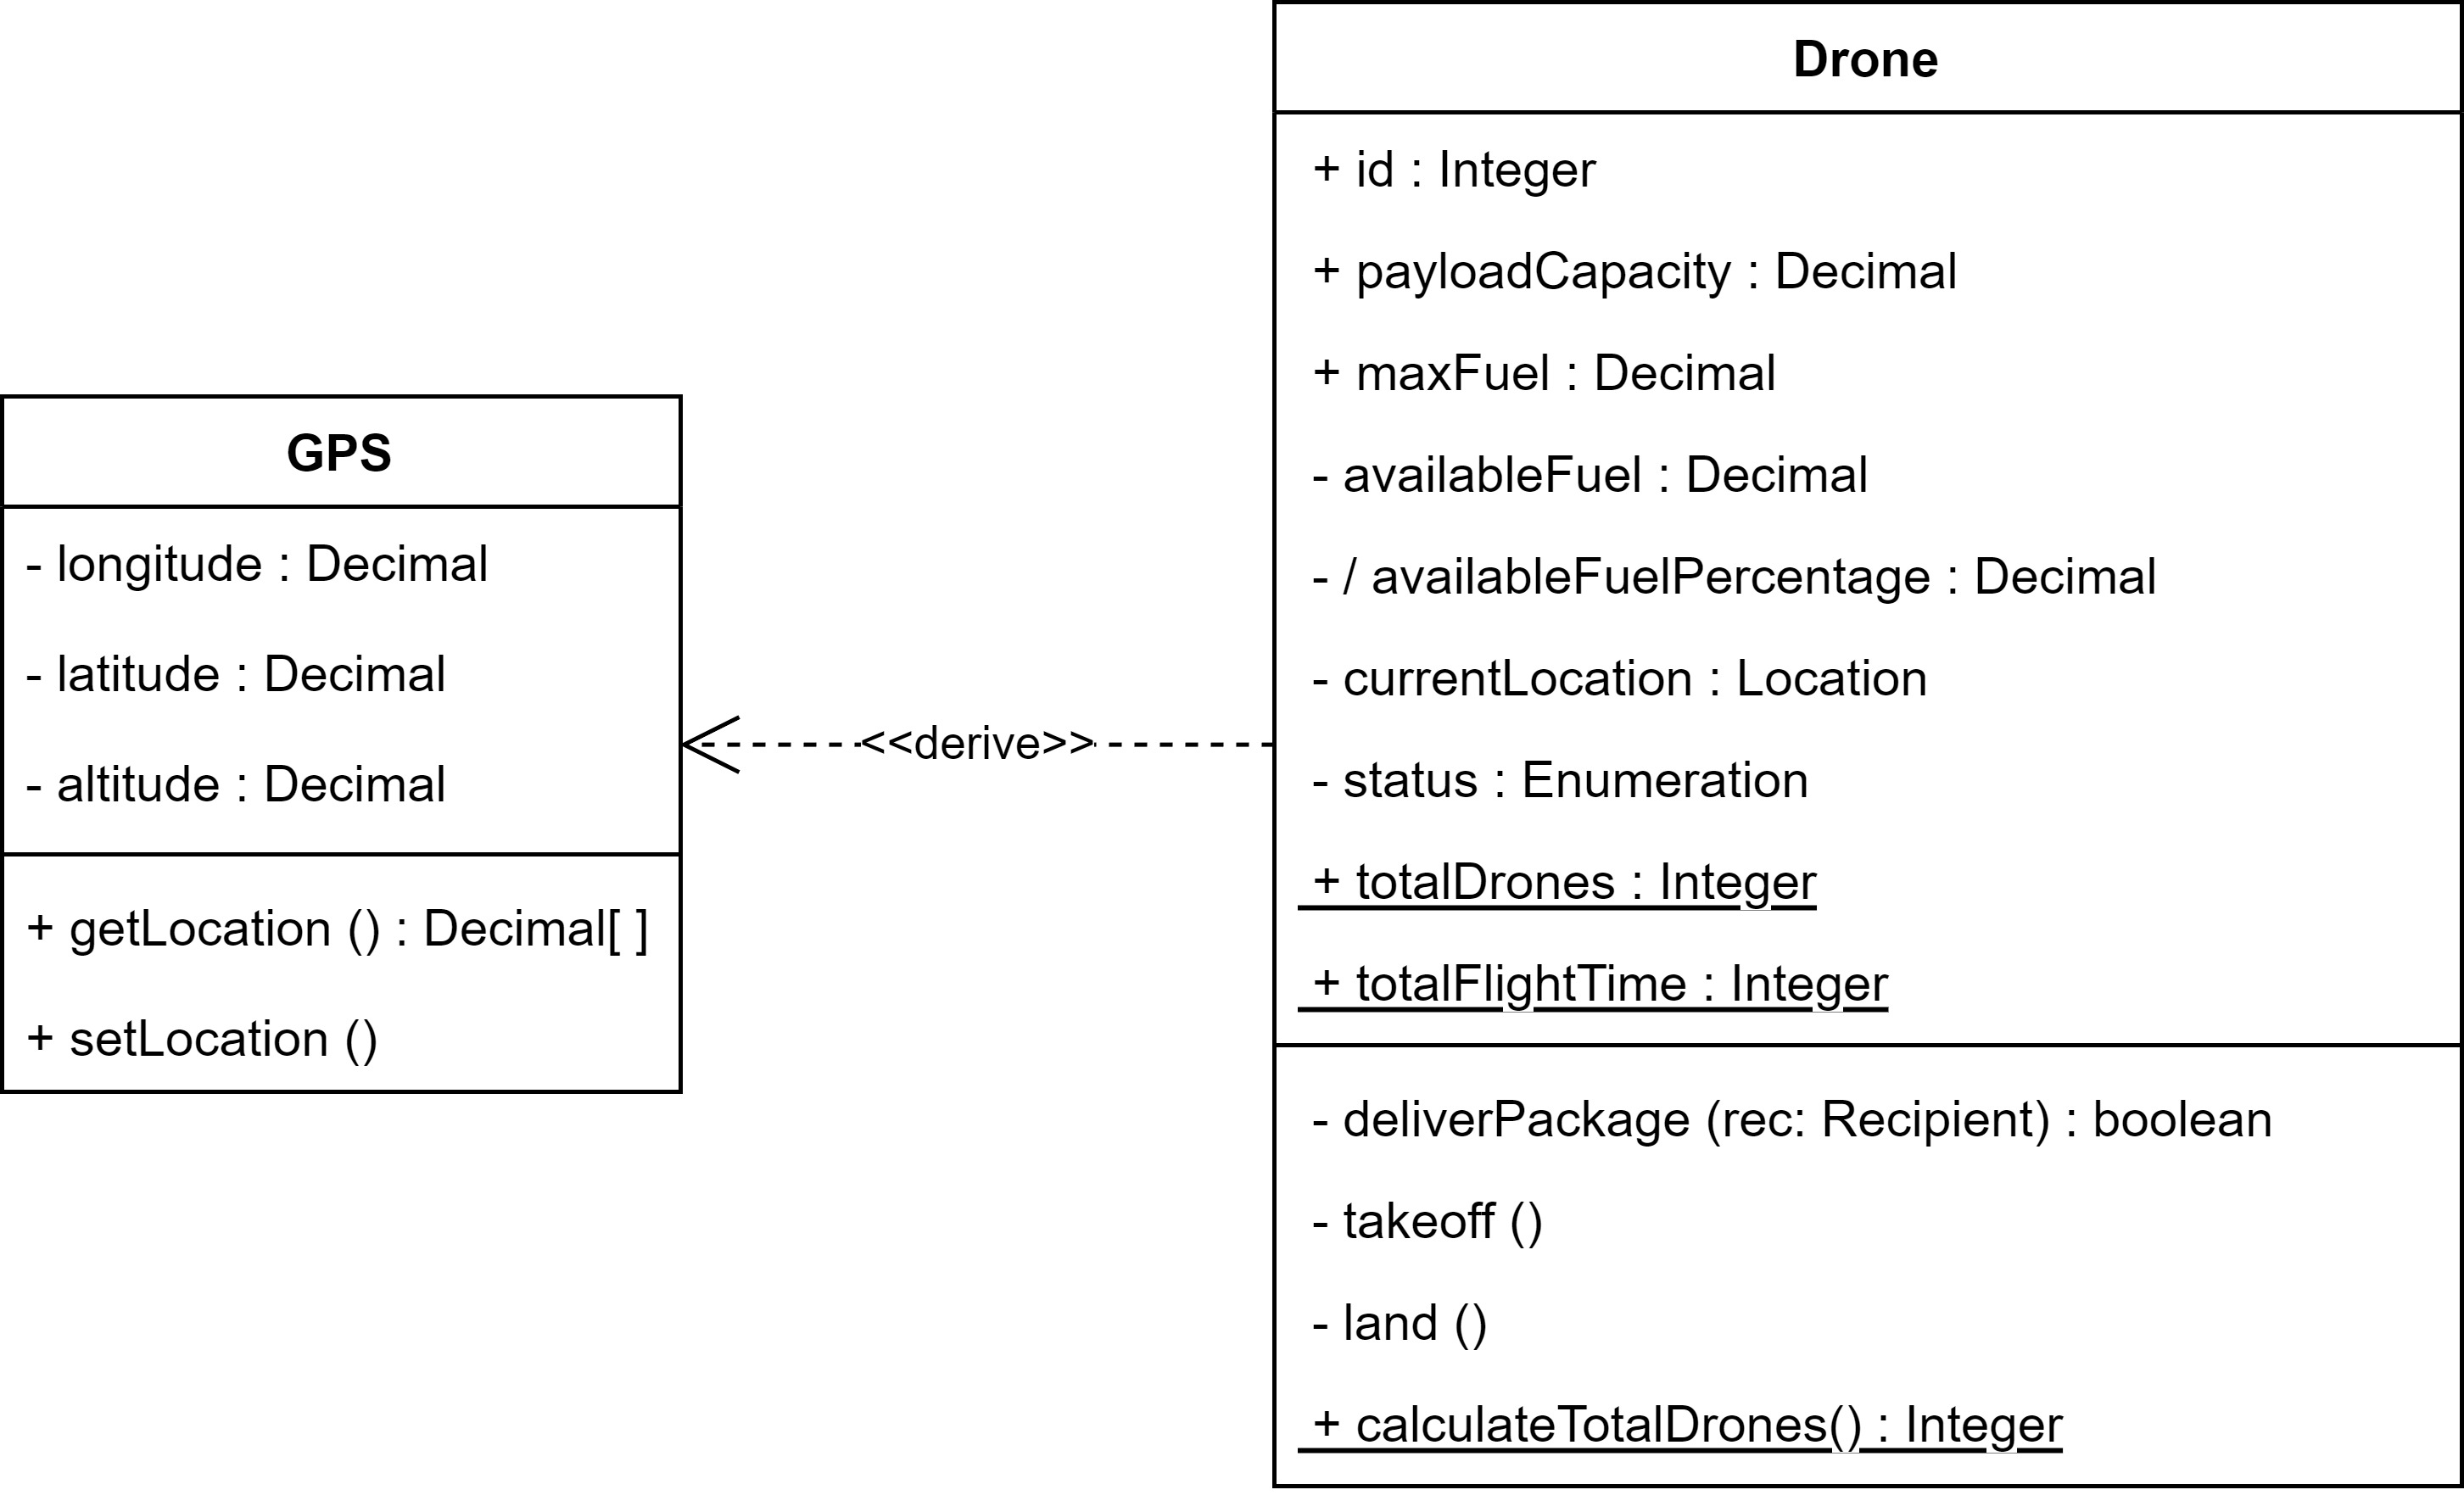
\includegraphics[width=0.8\textwidth]{figures/dependencies/derive.jpg}
	\captionof{figure}[Example abstraction]{Example of a derive abstraction}
	\label{fig:derive_example}
\end{minipage}

In Figure \ref{fig:derive_example}, an example of a dependency relationship between the \texttt{Drone} class and the \texttt{GPS} class is displayed. 
The \texttt{GPS} class contains the private attributes \texttt{latitude}, \texttt{longitude}, and \texttt{altitude}, which store information about the drone's current location. It also has the public operations \texttt{getLocation()} and \texttt{setLocation()}, which allow the Drone class to retrieve and update the location information provided by the GPS class.
This dependency can be represented with a <<derive>> stereotype, as the drone calculates its location based on the information provided by the GPS.

The Drone class depends on the GPS class for accurate location data, as it is essential for the drone to be able to determine its position and navigate to the desired location. To retrieve the current location, the Drone class calls the \texttt{getLocation()} operation of the GPS class and stores the returned location in its \texttt{location} attribute. The Drone class can then use this information to perform actions such as flying to a specific location or avoiding obstacles.

This dependency between the Drone and GPS classes can be represented with a \texttt{<<derive>>} stereotype, as the drone calculates its location based on the information provided by the GPS. 
The GPS class is the supplier of this information, and the Drone class is the client that depends on it. 
Without the GPS, the drone would be unable to determine its location and would be unable to perform its intended functions.

\vspace{1em}
\begin{minipage}{\linewidth}
	\centering
	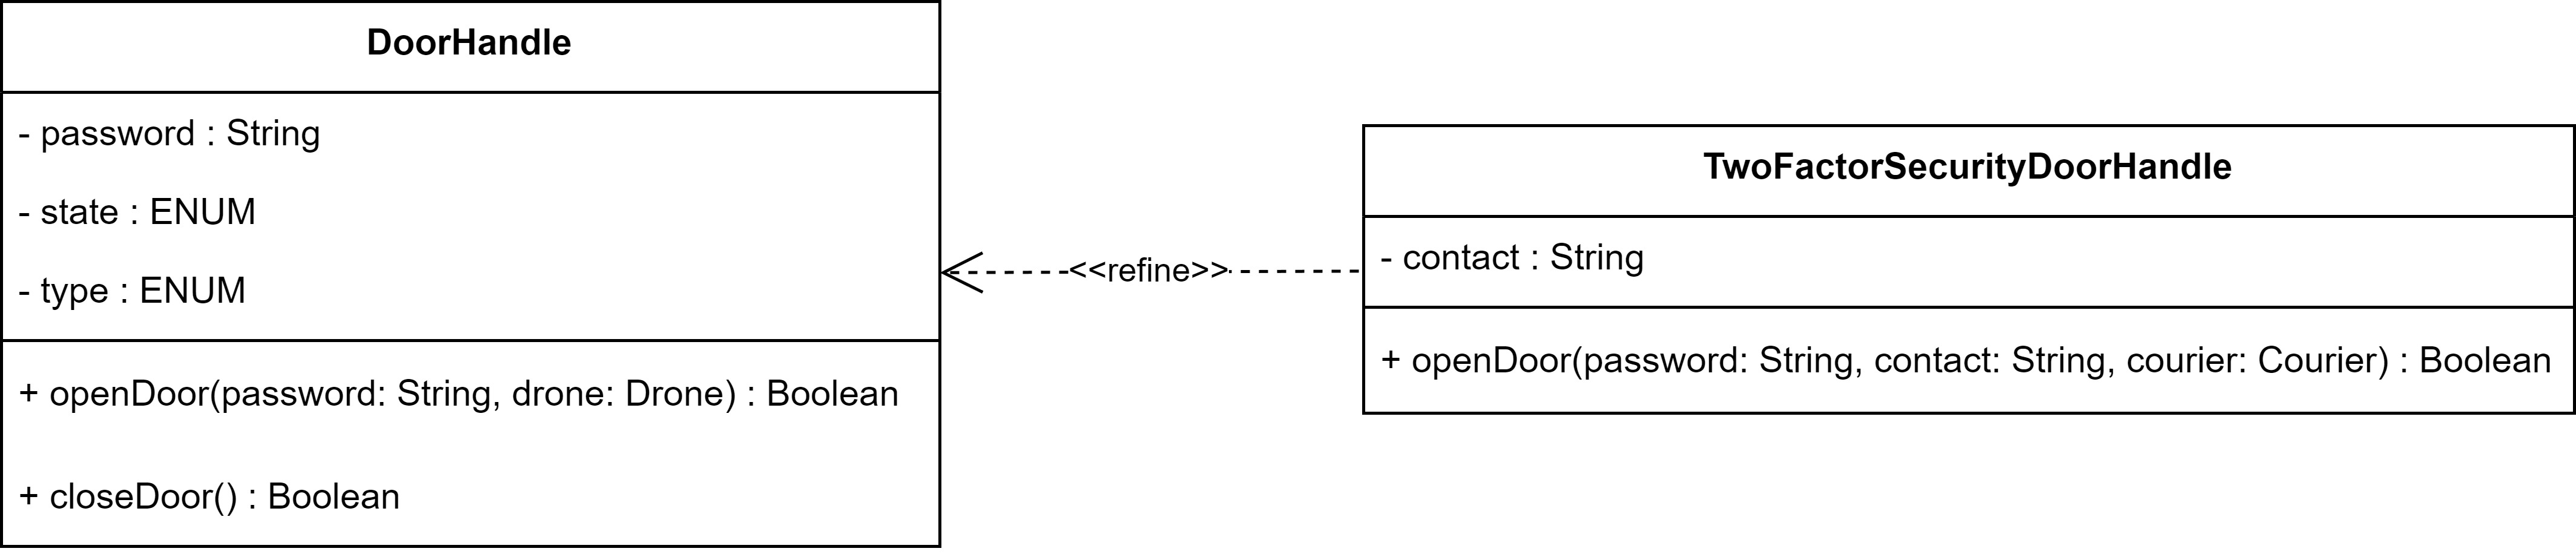
\includegraphics[width=0.8\textwidth]{figures/dependencies/refine.jpg}
	\captionof{figure}[Example abstraction]{Example of a refine abstraction}
	\label{fig:refine_example}
\end{minipage}

In Figure \ref{fig:refine_example}, an example of a refinement relationship between the \texttt{DoorHandle} class and the \texttt{TwoFactorSecurityDoorHandle} class is displayed.

The \texttt{DoorHandle} class, which was previously used by the drone to open and close doors as part of its delivery tasks, has been refined by the \texttt{TwoFactorSecurityDoorHandle} class to add an extra layer of security. The \texttt{TwoFactorSecurityDoorHandle} class has a private attribute \texttt{contact} that stores the phone number, email address, or recipient's ID in the delivery app.

When the drone calls the new \texttt{closeDoor} operation of the \texttt{TwoFactorSecurityDoorHandle} class, the recipient will receive a notification that they must answer, in addition to the password that the drone inputs, for the door to be opened. This added security measure ensures that only the drone with the intended package can unlock the door.

The \texttt{TwoFactorSecurityDoorHandle} class is shown as the client element in the refinement relationship, which is depicted with a dashed line with an open arrow pointing from the \texttt{TwoFactorSecurityDoorHandle} class to the \texttt{DoorHandle} class. The stereotype \texttt{<<refine>>} is added to the relationship to indicate that the \texttt{TwoFactorSecurityDoorHandle} class refines the \texttt{DoorHandle} class.

\section{Substitution}
%In UML, a substitution dependency is a relationship between classifiers that allows one classifier (the client) to be used in place of another classifier (the supplier) at runtime.
%The client classifier must meet all requirements specified by the supplier, including implementing interfaces and having corresponding ports. 
%The substitution dependency is depicted in a UML diagram with a dashed line and open arrow pointing from the client to the supplier, and the stereotype \texttt{<<substitute>>} added to the relationship. 
%Only classifiers, such as classes or components, can be connected in a substitution dependency. 
%Substitution dependencies can be used when inheritance is not possible or appropriate, for example, if the supplier classifier is part of a third-party library and cannot be modified. 
%The client and supplier classifiers in a substitution dependency do not need to have similar base structures, allowing for more flexible and complex designs. \cite[p. 165]{uml}

In UML, a substitution dependency is a relationship between classifiers where one classifier (the client) can replace another classifier (the supplier) at runtime. 
It is depicted with a dashed line with an open arrow pointing from the client to the supplier and the stereotype \texttt{<<substitute>>}. \cite[p.165]{uml}


One common use case for substitution dependencies is when a classifier is being replaced or upgraded with a new version, but the new version needs to maintain compatibility with the original classifier. 
For example, the drone delivery system originally used a fleet of traditional drones for deliveries. As the company develops and deploys a new line of robots that are capable of performing the same tasks as the drones, a substitution dependency may be used to indicate that the robots can be used as a substitute for the drones.

\vspace{1em}
\begin{minipage}{\linewidth}
	\centering
	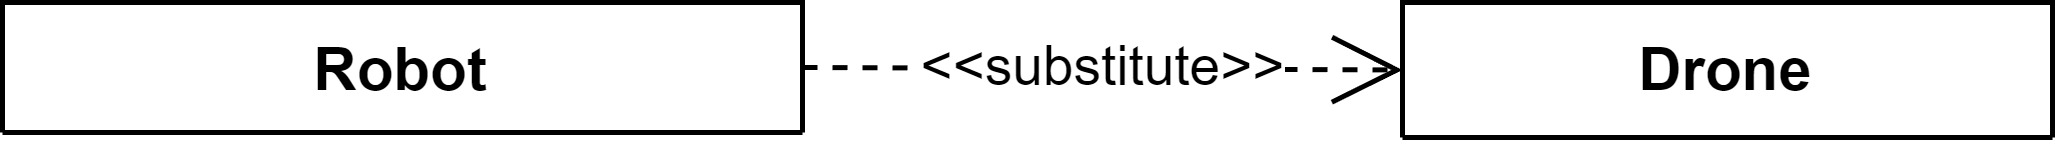
\includegraphics[width=0.8\textwidth]{figures/dependencies/substitute.jpg}
	\captionof{figure}[Example substitution]{Example of a substitution}
	\label{fig:substitution_example}
\end{minipage}

In Figure \ref{fig:substitution_example}, an example of a substitution relationship between the \texttt{Drone} class and the \texttt{Robot} class is displayed.
The \texttt{Drone} class has been designated as the contract classifier, which means that it specifies a set of obligations that must be fulfilled by any substituting classifiers. 
In this case, the \texttt{Robot} class has been identified as a substituting classifier, which means that it can be used in place of the \texttt{Drone} class wherever instances of the \texttt{Drone} class are expected.
To fulfill the obligations specified by the \texttt{Drone} class, the \texttt{Robot} class must implement all interfaces and ports that are required by the \texttt{Drone} class. 
For example, the \texttt{Drone} class requires the implementation of a \texttt{deliverPackage()} operation, which must also be implemented by the \texttt{Robot} class to be used as a valid substitution.


\section{Realization}
%A realization dependency relationship indicates that the client model element is an implementation of the supplier model element, and the supplier model element is the specification.
%A realization relationship can be used to model the relationship between a class and an interface, a component and a class, or a component and an interface. 
%It represents the implementation of a contract defined by the supplier element and indicates that the client element provides the behavior specified by the supplier element.
%In UML2 a realization relationship is depicted as a solid line with a hollow triangle arrowhead pointing from the client element to the supplier element.
%Before UML2 the usual notation of dependencies, using a dashed line with an open arrow, was used as an alternative. \cite[p. 164]{uml}
%
%An example of the realization relationship will be presented in the Interface chapter.

A realization relationship in UML class diagrams indicates that a client model element (e.g. class, component) is an implementation of a supplier model element (e.g. interface, abstract class). 
It represents the implementation of a contract defined by the supplier element, and is depicted as a solid line with a hollow triangle arrowhead pointing from the client to the supplier.
In earlier versions of UML, a dashed line with an open arrow was used as an alternative. 

An example of the realization relationship will be presented in the Interface chapter.


%TODO in appendix?
\section{Multiple dependencies}
In cases where a client has a dependency on several suppliers, a connector (represented as a small black dot) can be used to model the dependency.  \cite[p. 160]{uml}
In the following Figure \ref{fig:multiple_dependencies_example} an example of possible multiple dependencies is displayed.

\vspace{1em}
\begin{minipage}{\linewidth}
	\centering
	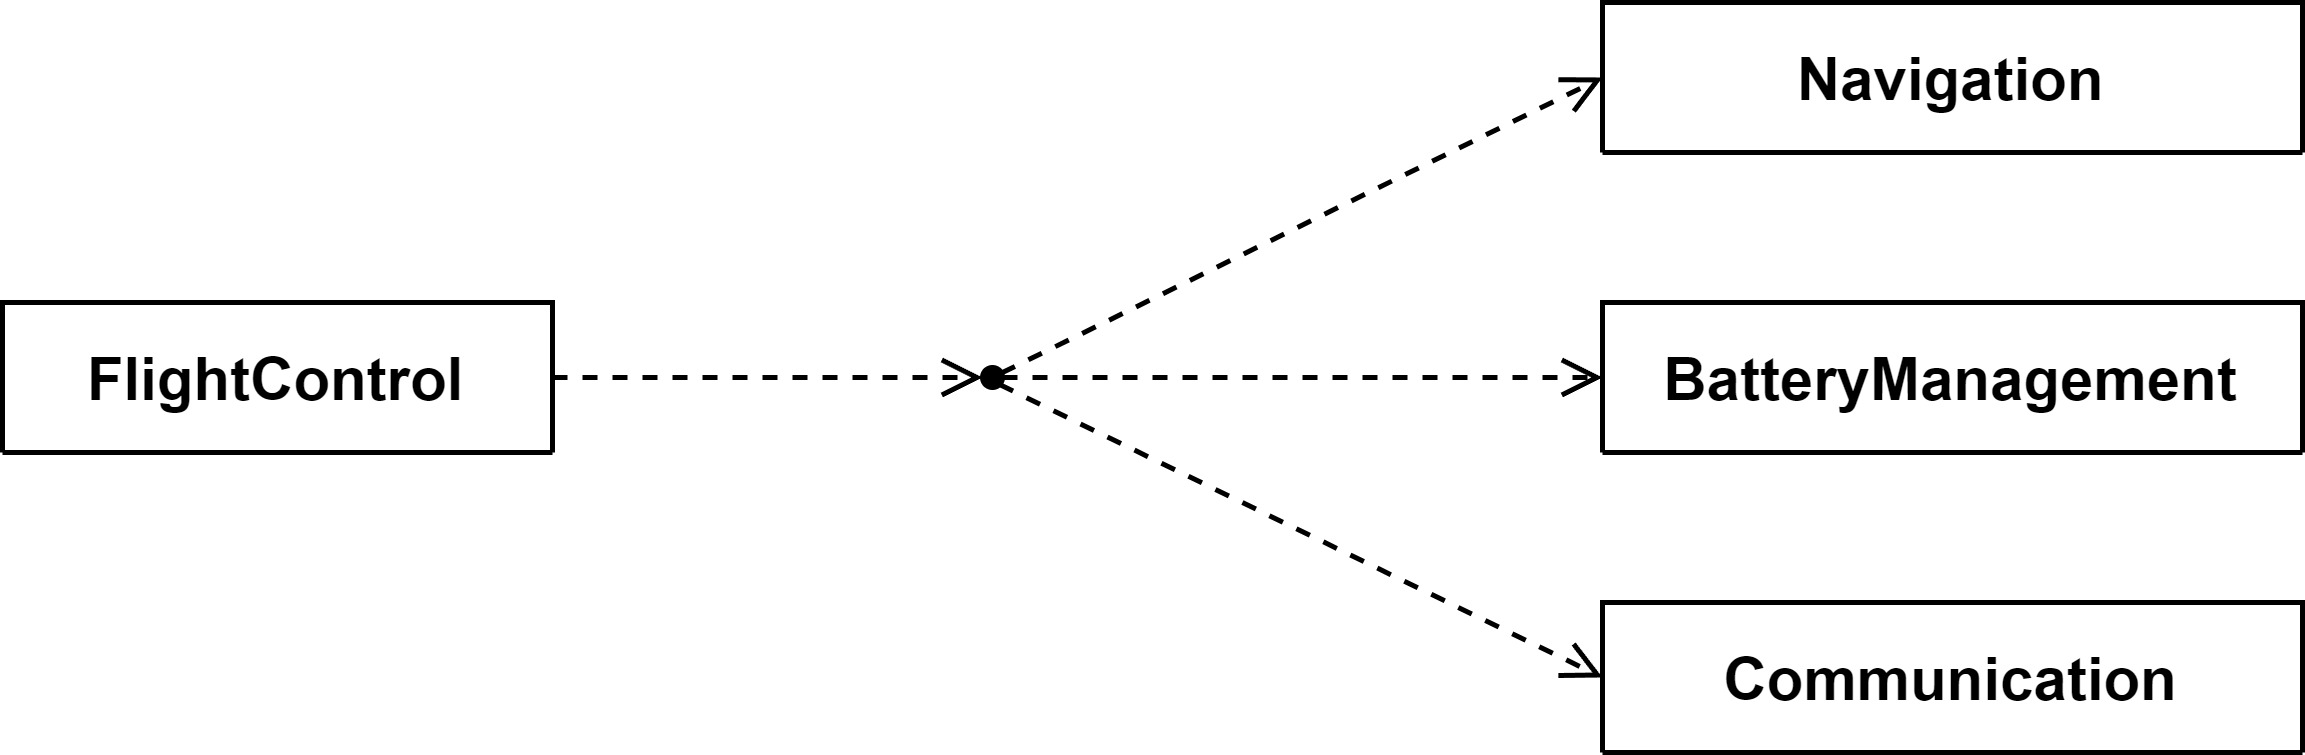
\includegraphics[width=0.7\textwidth]{figures/dependencies/multiple_dependencies.jpg}
	\captionof{figure}[Example multiple dependency]{Example of a multiple dependency}
	\label{fig:multiple_dependencies_example}
\end{minipage}

For the class \texttt{FlightControl} to work properly, it is dependent on the classes \texttt{Navigation}, \texttt{BatteryManagement}, and \texttt{Communication}.
Furthermore, the way the classes are dependent can be elaborated by stereotypes and added notes.

\section{Interface}

An interface is a type of classifier that represents a set of related behaviors that a class or component must implement to conform to the interface. 
An interface defines a set of abstract operations, which are public and do not have any implementation.
Interfaces are represented by a classifier rectangle with the stereotype \texttt{«interface»} at the top, followed by the name of the interface. 
The operations and attributes of the interface are listed inside the rectangle. \cite[p. 130-131]{uml}

There are two equivalent ways of displaying an interface relationship which are shown in the following Figure \ref{fig:interface_notation}:

\begin{minipage}{\linewidth}
	\centering
	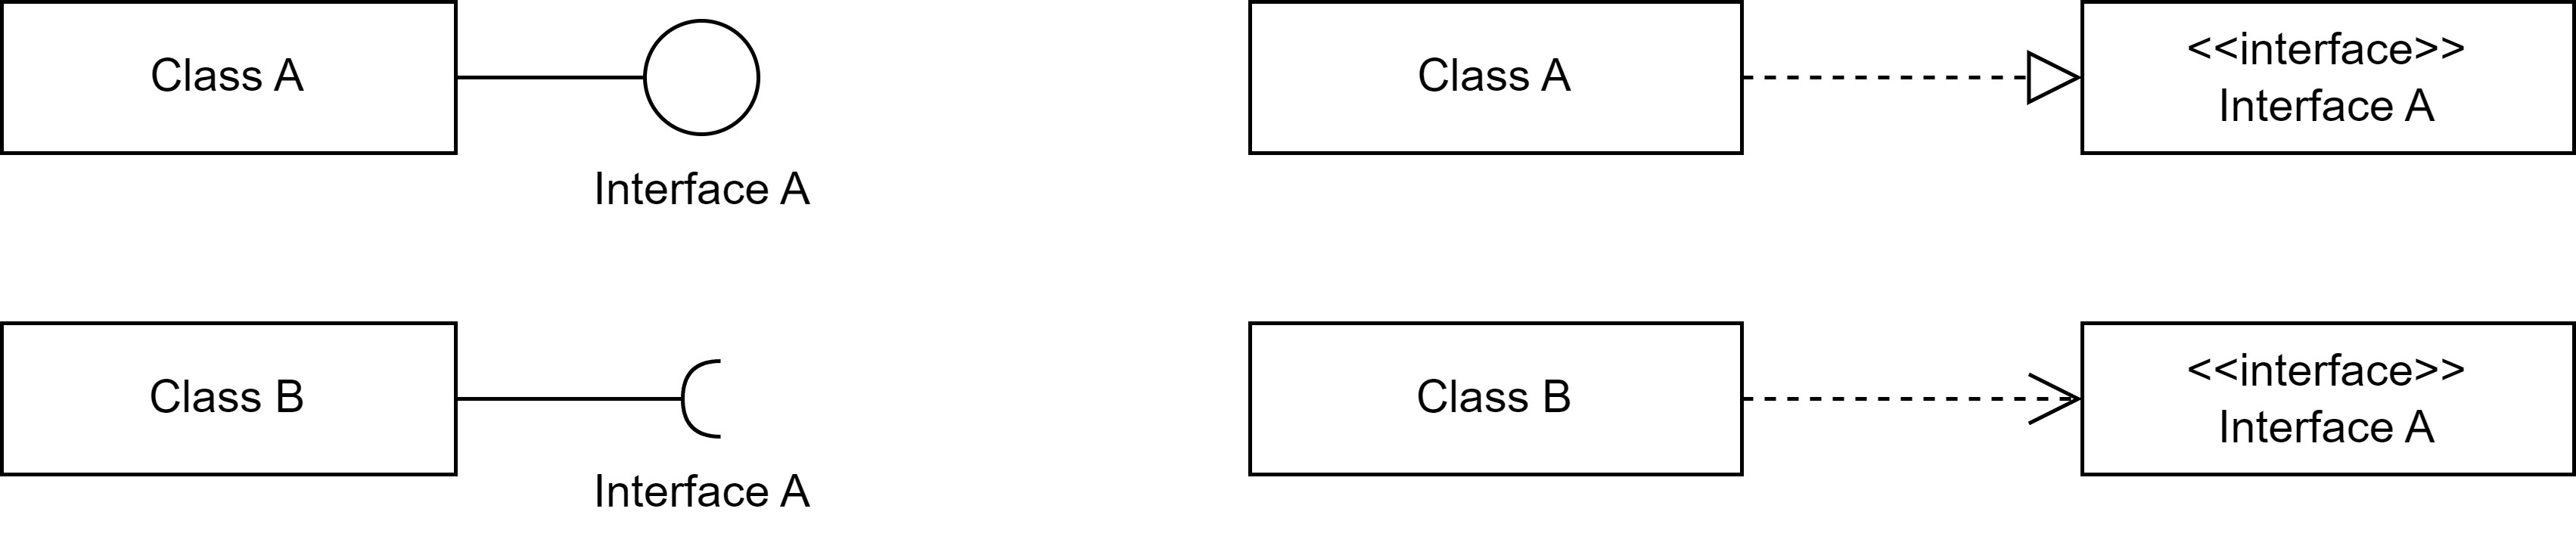
\includegraphics[width=0.8\textwidth]{figures/interface/Interface_Notation.jpg}
	\captionof{figure}[Notation of an interface relationship]{Notation of an interface relationship}
	\label{fig:interface_notation}
\end{minipage}

The left side shows the lollipop and the right side the arrow notation.
The first row displays the implementation of the interface with the class.
The second row displays that the class requires an implementation of this interface. \cite[p. 129]{uml}
In the following the arrow notation will be used.
                
\begin{minipage}{\linewidth}
	\centering
	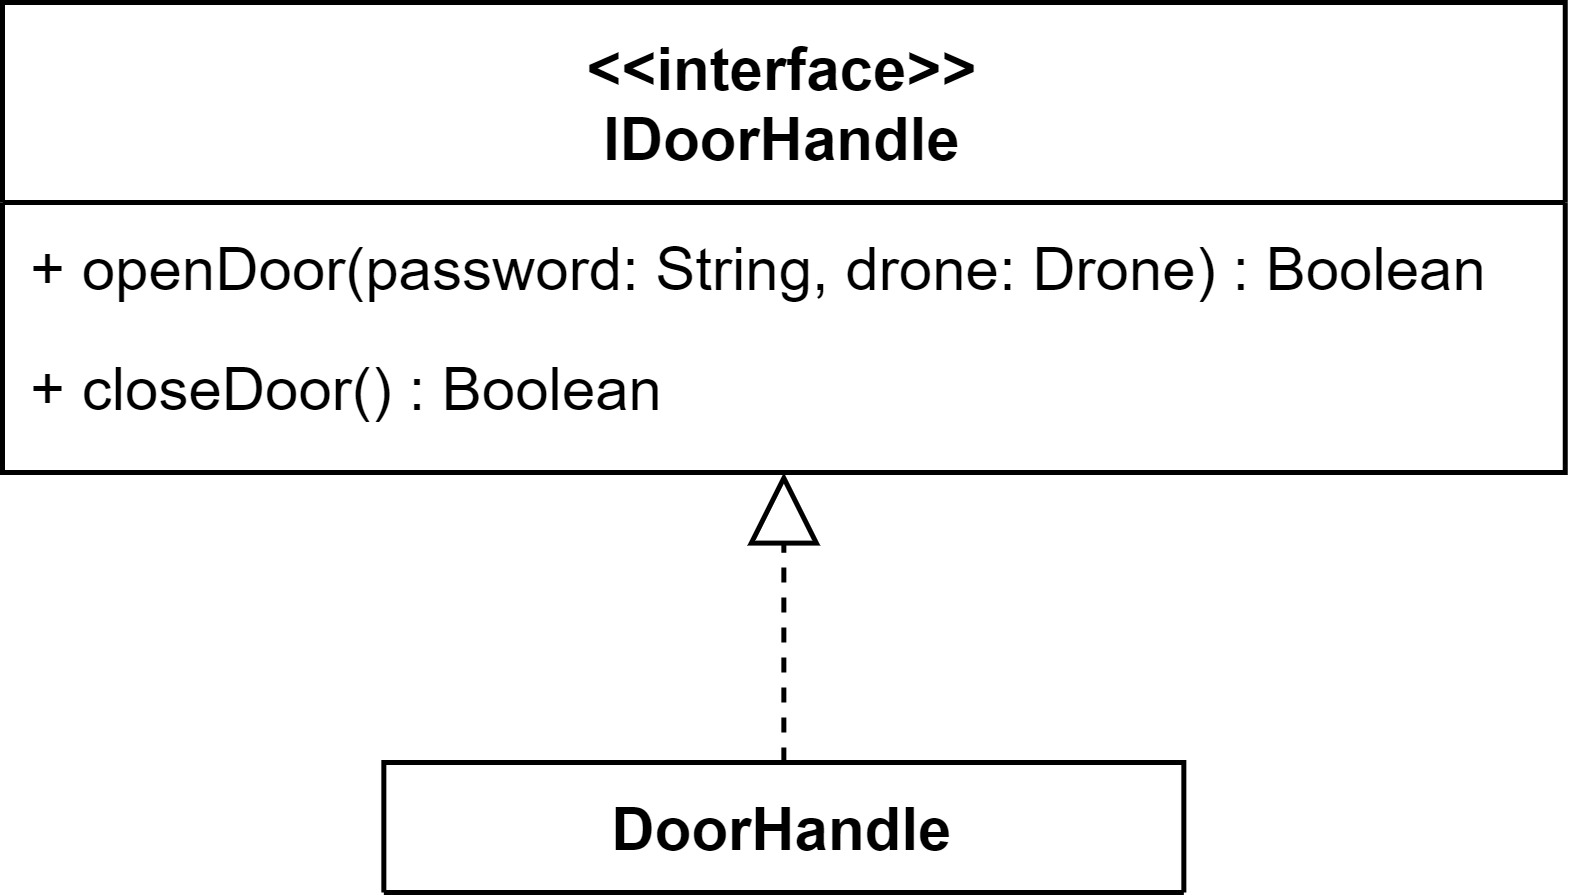
\includegraphics[width=0.6\textwidth]{figures/interface/doorhandle_interface.jpg}
	\captionof{figure}[Example interface]{Example of a DoorHandle interface}
	\label{fig:interface_example}
\end{minipage}

An example of an interface is shown in Figure \ref{fig:interface_example}, where the \texttt{IDoorHandle} interface has a realization relationship with the \texttt{DoorHandle} class.
The \texttt{DoorHandle} class implements the \texttt{openDoor()} and \texttt{closeDoor()} operations defined in the interface, allowing for flexibility in the implementation.
For instance, a different version of the \texttt{DoorHandle} class that also implements these operations could be used in place of the original.
Interfaces in UML allow for easy substitution of different class implementations while maintaining the same set of required operations.


\vspace{1em}
\begin{minipage}{\linewidth}
	\centering
	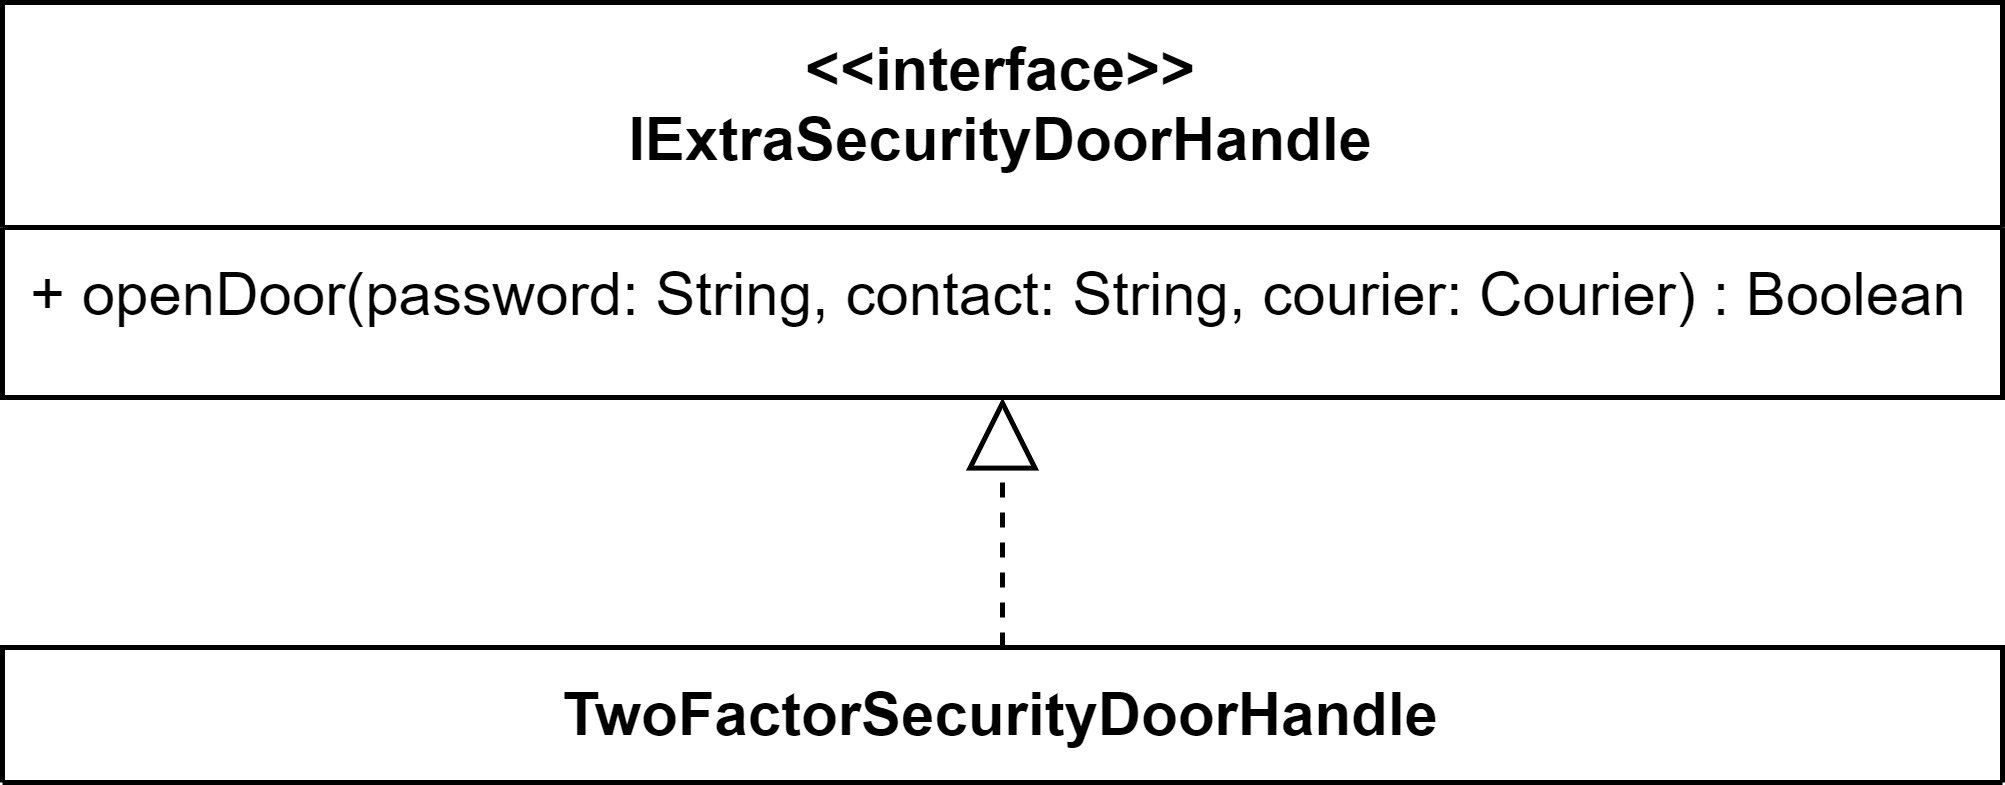
\includegraphics[width=0.7\textwidth]{figures/interface/doorhandle_sec_interface.jpg}
	\captionof{figure}[Example interface]{Example of an ExtraSecurityDoorHandle interface}
	\label{fig:interface2_example}
\end{minipage}

In Figure \ref{fig:interface2_example}, another example of an interface relationship is shown. 
The \texttt{IExtraSecurityDoorHandle} interface allows for multiple different implementations of secure DoorHandles to be easily swapped in and out. The \texttt{TwoFactorSecurityDoorHandle} class implements the \texttt{openDoor()} operation of the \texttt{IExtraSecurityDoorHandle} interface.


%TODO kürzen, damit alles auf 2 Seiten passt
\chapter{Inheritance}
In UML class diagrams, inheritance is a relationship between two classes in which one class (the subclass or derived class) is a specialization of the other class (the superclass or base class). 
This means that the subclass inherits the attributes, operations and associations of the superclass, and can add additional of its own.
Inheritance is displayed by a solid line with a closed, non filled, arrow pointing from the subclass to the superclass.
The two ways of designing inheritance relationships are described in the following.

Generalization is a term used to describe the process of creating a superclass from one or more subclasses. 
This is typically done to identify common attributes and behaviors shared by the subclasses and to create a more generalized, abstract representation of these concepts. \cite[p. 69-70] {seidl2015uml} \cite{ibm_generalization}


\vspace{1em}
\begin{minipage}{\linewidth}
	\centering
	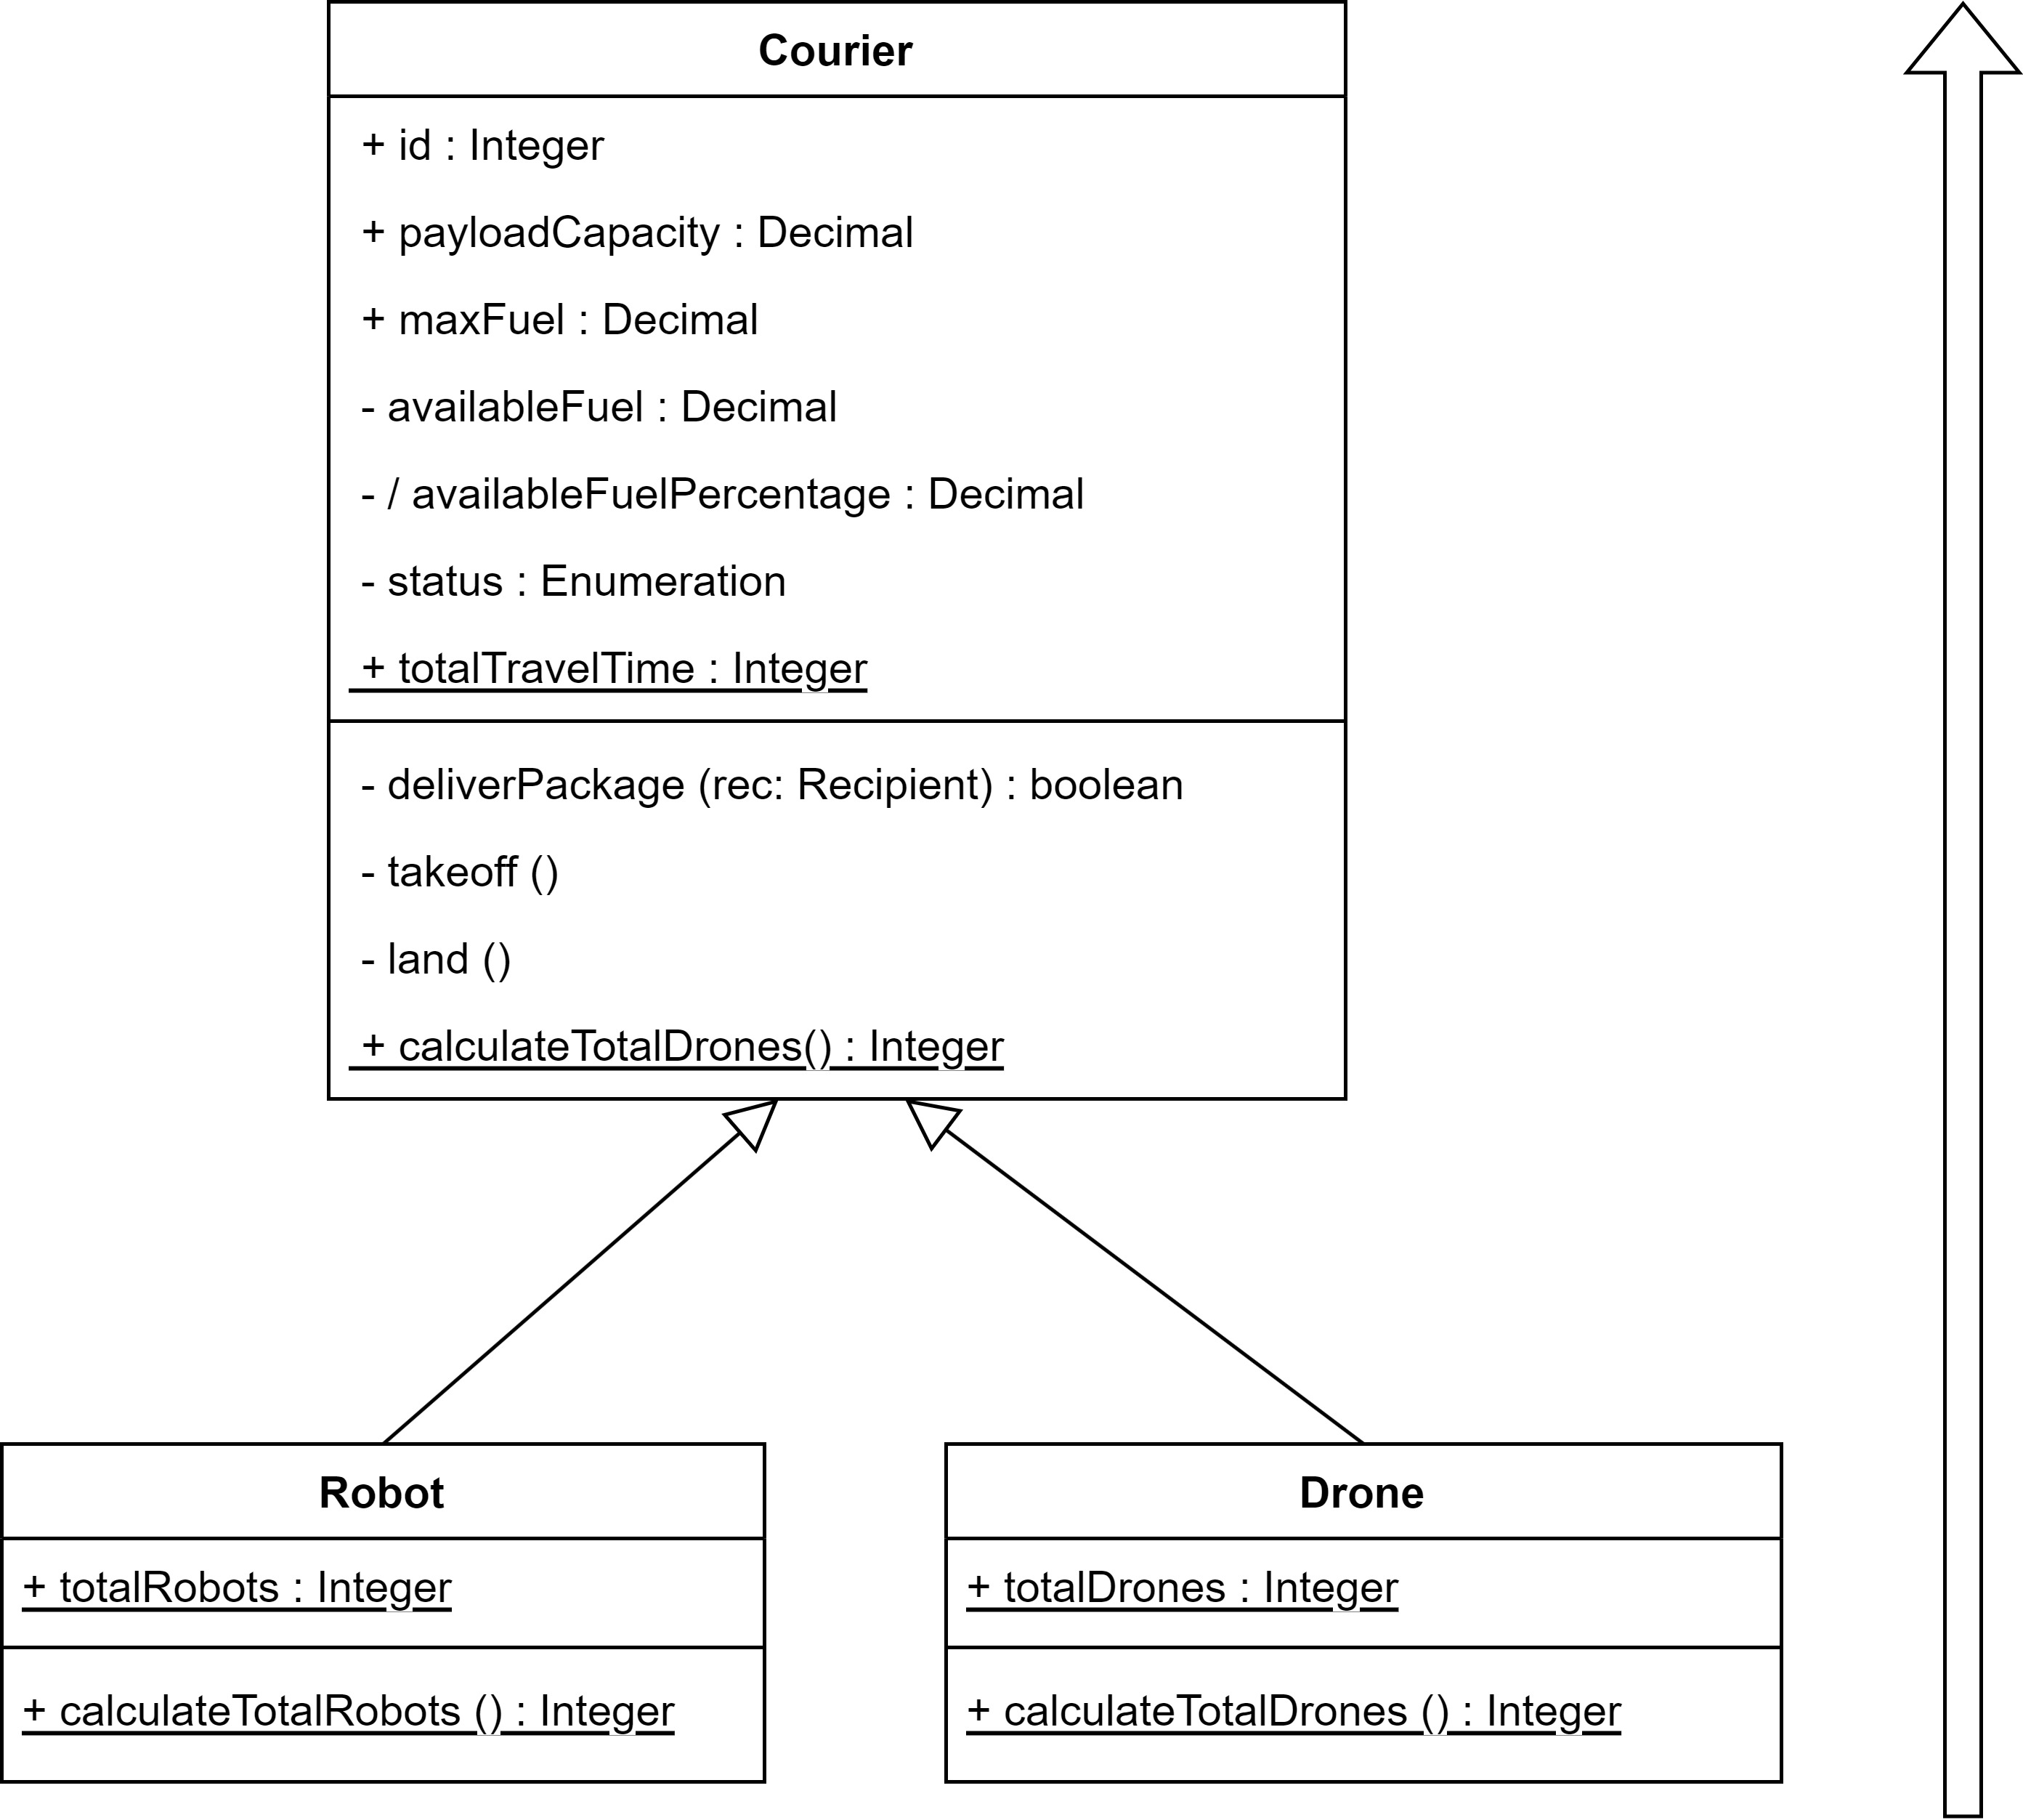
\includegraphics[width=0.7\textwidth]{figures/inheritance/generalization.jpg}
	\captionof{figure}[Example generalization]{Example of generalization}
	\label{fig:generalization}
\end{minipage}

In Figure \ref{fig:generalization}, an example of inheritance and generalization is shown. 
The class \texttt{Robot} has been added to the system as an additional form of transportation. 
Since the classes \texttt{Robot} and \texttt{Drone} have many attributes and operations in common, they have been extracted into a superclass, the \texttt{Courier}.
This means that both subclasses inherit the attributes, operations, and associations of the superclass. 
The superclass \texttt{Courier} has replaced the \texttt{Drone} class in its previous relationships that have been shown in prior examples.
The arrow on the right side indicates that the superclass is formed from its two subclasses, which have been designed before the superclass.



Specialization is the process of creating a subclass from a superclass. This is typically done to add more specific attributes and behaviors to the subclass, or to specialize the subclass for a particular purpose.

In the following Figure \ref{fig:specialization}, an example of specialization is depicted. The figure illustrates that, given the existence of a superclass, the subclasses can be derived from it, resulting in a specialization relationship. 
The arrow on the right side of the figure indicates that the subclasses, in this case \texttt{Drone} and \texttt{Robot}, are derived from the superclass \texttt{Courier}, which was designed prior to them. 
This inheritance relationship allows the subclasses to inherit the attributes, operations, and associations of the superclass.

\vspace{1em}
\begin{minipage}{\linewidth}
	\centering
	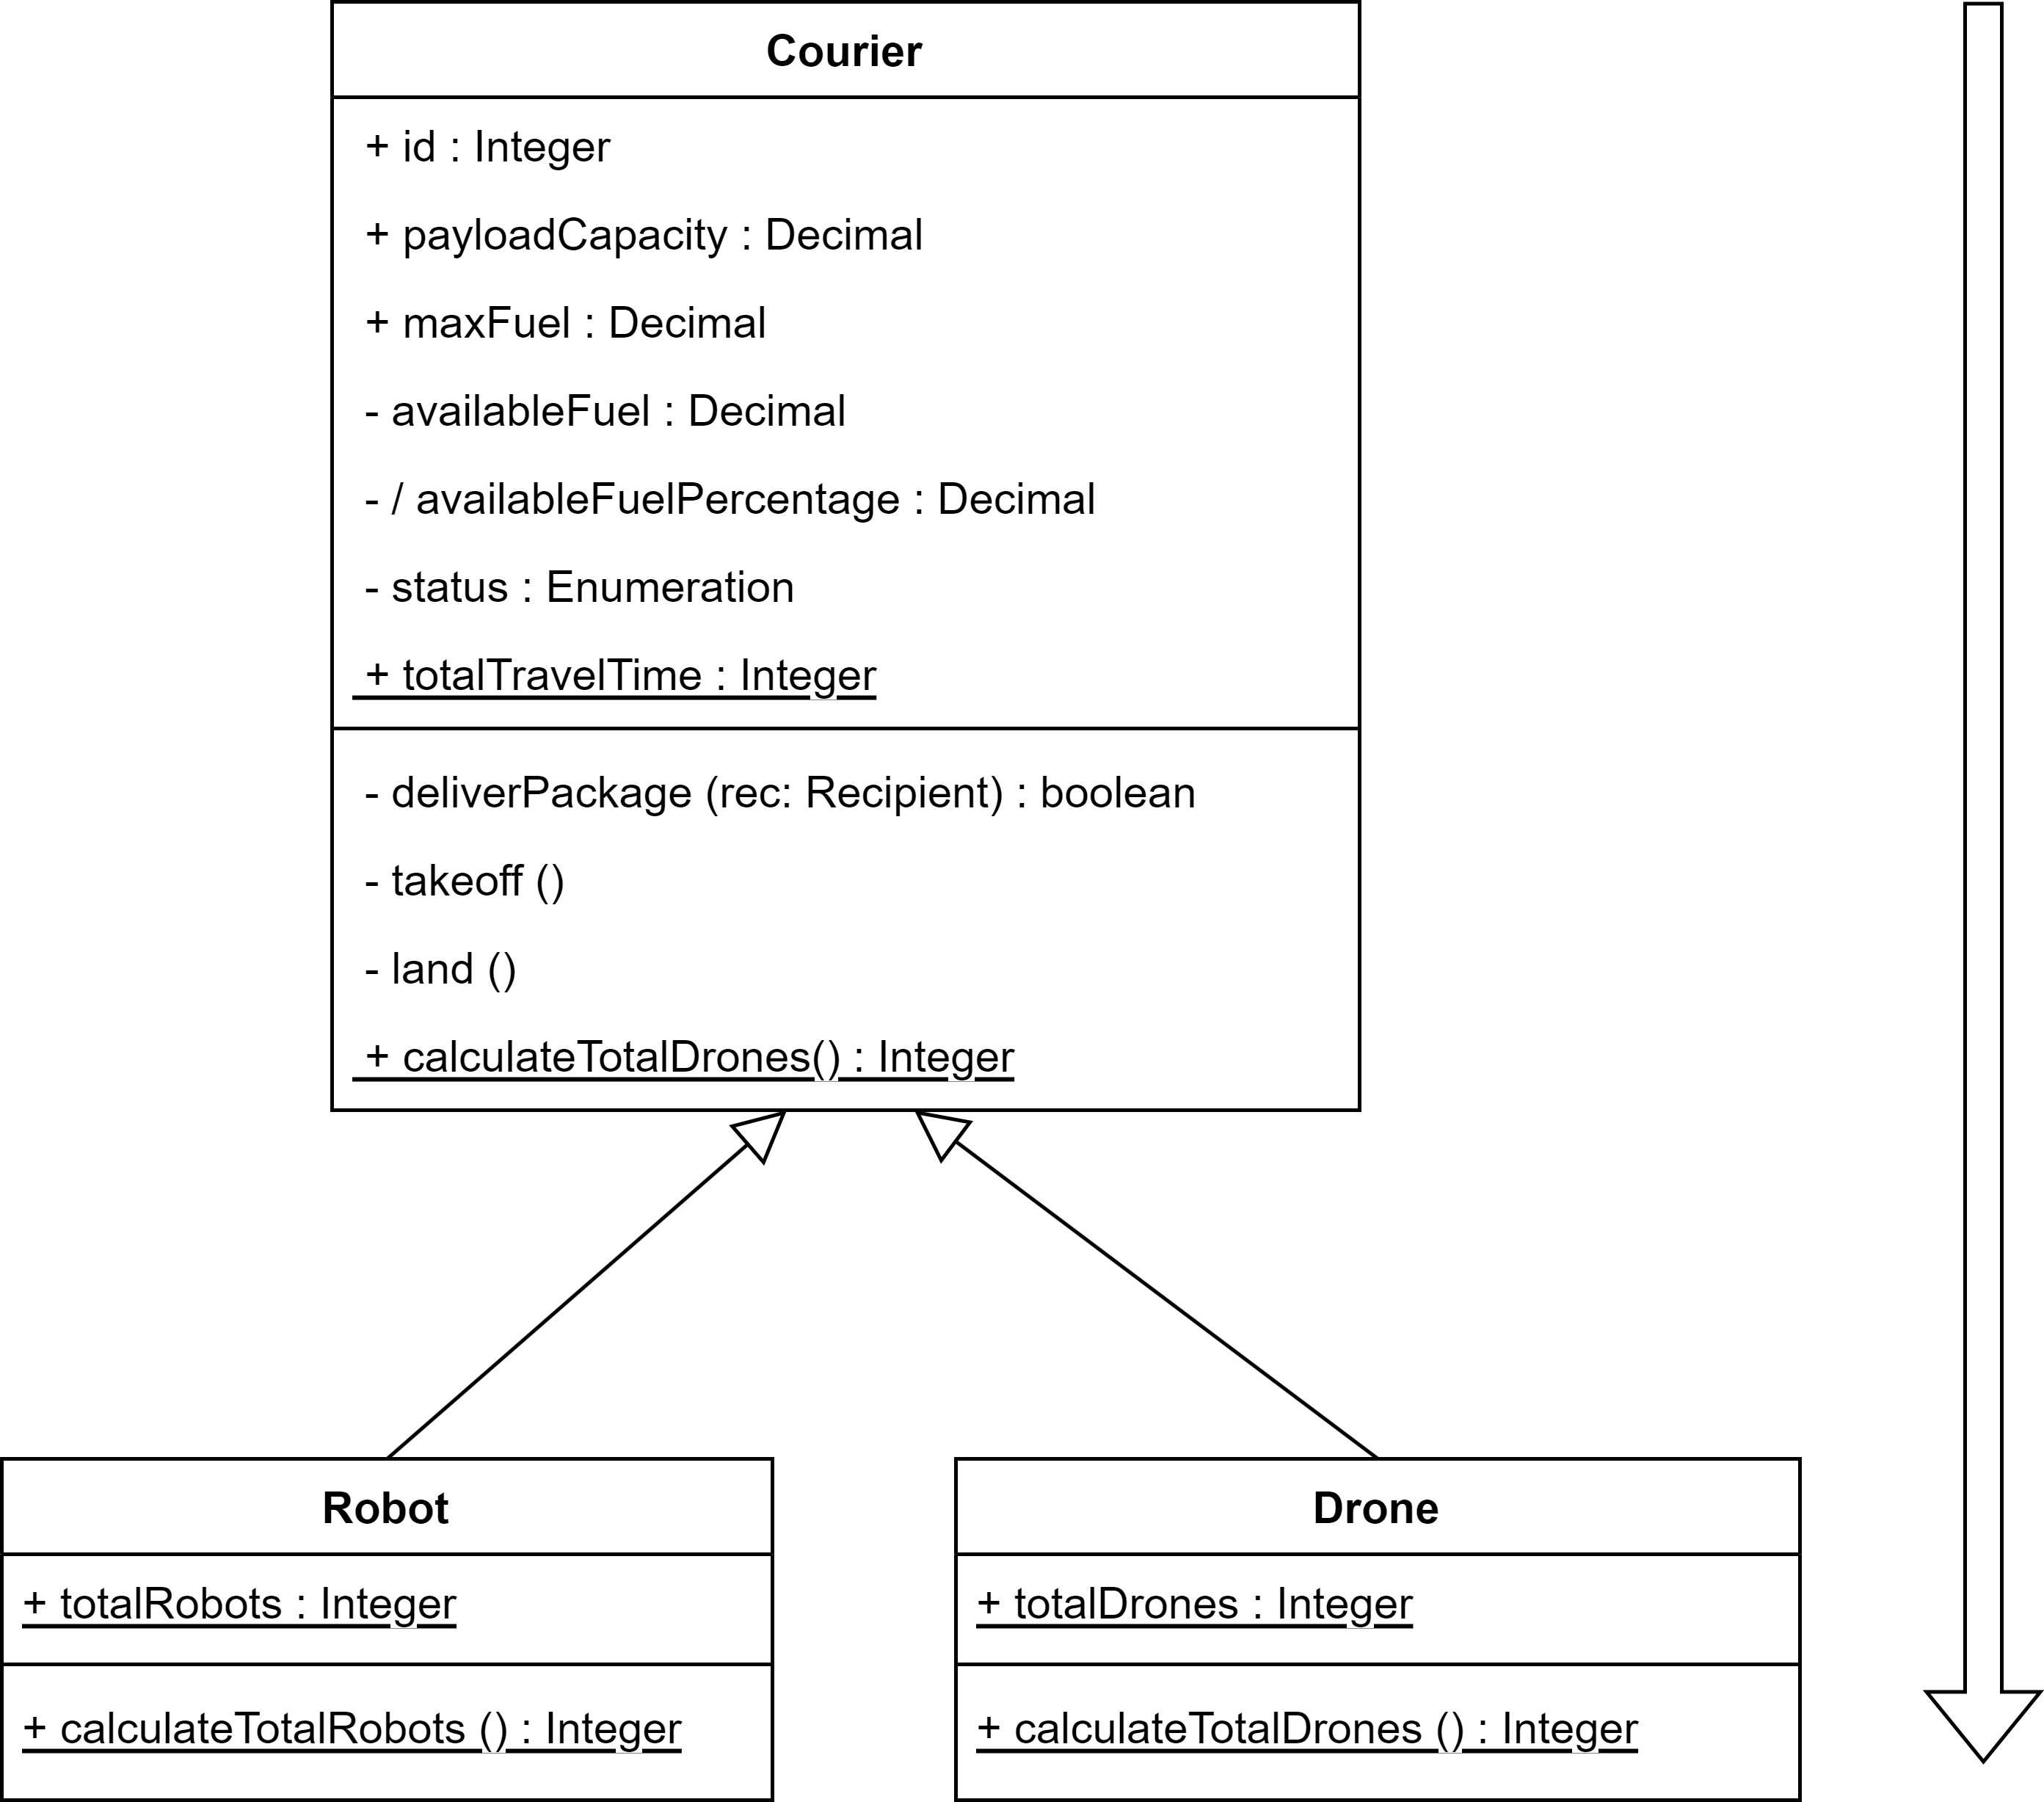
\includegraphics[width=0.7\textwidth]{figures/inheritance/specialization.jpg}
	\captionof{figure}[Example specialization]{Example of specialization}
	\label{fig:specialization}
\end{minipage}

UML also allows multiple inheritance, which means classes can have multiple superclasses. \cite[p. 71] {seidl2015uml}

\chapter{Resumee and outlook}


In Figure \ref{fig:full}, a comprehensive class diagram for a drone delivery system is presented, incorporating all the examples discussed in this paper except for the flight control system (which involves multiple dependencies). 
This diagram illustrates the various classes and relationships involved in the delivery process, with Levin's [add citation] paper as the starting point. 
However, it is worth noting that this diagram only represents the delivery side of the system and could be further expanded to include logistics such as package acquisition and packaging.

One of the main benefits of using UML class diagrams is their ability to visually represent the relationships and interactions between different classes in a system. 
This can help developers better understand the overall structure and design of the system, as well as identify potential areas for improvement or optimization.

In addition, the use of relationships, such as inheritance and generalization, can help to reduce redundancy and improve maintainability by allowing common functionality to be shared among multiple classes. This can also facilitate the reuse of code and make it easier to add new features or functionality to the system.

Overall, the use of UML class diagrams and complex relationships can help to improve the design and development of software systems, leading to more efficient and effective implementations.

%TODO in Appendix?
\begin{figure}[p]
	\centering
	\rotatebox{90}{\includegraphics[width=\textheight]{figures/full/full.jpg}}
	\captionof{figure}[Full diagram]{Full diagram}
	\label{fig:full}
\end{figure}



\backmatter
%\listoftodos %remove if no longer needed

\printnoidxglossaries

% ACHTUNG: ursprüngl: alpha, aber das erzeugt keine Links
%\bibliographystyle{wmaainf}
%\bibliographystyle{alpha}
%\bibliography{refs}
\printbibliography

\clearpage %\cleardoublepage

%-----------------------------------------------------------------------------------------------------------------

% remove if not needed
\appendix
%\pagenumbering{Alph}
\chapter{Supplemental Information}\label{app:supplemental-information}
Hier könnte Ihr Anhang stehen!


%-----------------------------------------------------------------------------------------------------------------


\end{document}